\documentclass[twoside]{book}

% Packages required by doxygen
\usepackage{fixltx2e}
\usepackage{calc}
\usepackage{doxygen}
\usepackage[export]{adjustbox} % also loads graphicx
\usepackage{graphicx}
\usepackage[utf8]{inputenc}
\usepackage{makeidx}
\usepackage{multicol}
\usepackage{multirow}
\PassOptionsToPackage{warn}{textcomp}
\usepackage{textcomp}
\usepackage[nointegrals]{wasysym}
\usepackage[table]{xcolor}

% Font selection
\usepackage[T1]{fontenc}
\usepackage[scaled=.90]{helvet}
\usepackage{courier}
\usepackage{amssymb}
\usepackage{sectsty}
\renewcommand{\familydefault}{\sfdefault}
\allsectionsfont{%
  \fontseries{bc}\selectfont%
  \color{darkgray}%
}
\renewcommand{\DoxyLabelFont}{%
  \fontseries{bc}\selectfont%
  \color{darkgray}%
}
\newcommand{\+}{\discretionary{\mbox{\scriptsize$\hookleftarrow$}}{}{}}

% Page & text layout
\usepackage{geometry}
\geometry{%
  a4paper,%
  top=2.5cm,%
  bottom=2.5cm,%
  left=2.5cm,%
  right=2.5cm%
}
\tolerance=750
\hfuzz=15pt
\hbadness=750
\setlength{\emergencystretch}{15pt}
\setlength{\parindent}{0cm}
\setlength{\parskip}{3ex plus 2ex minus 2ex}
\makeatletter
\renewcommand{\paragraph}{%
  \@startsection{paragraph}{4}{0ex}{-1.0ex}{1.0ex}{%
    \normalfont\normalsize\bfseries\SS@parafont%
  }%
}
\renewcommand{\subparagraph}{%
  \@startsection{subparagraph}{5}{0ex}{-1.0ex}{1.0ex}{%
    \normalfont\normalsize\bfseries\SS@subparafont%
  }%
}
\makeatother

% Headers & footers
\usepackage{fancyhdr}
\pagestyle{fancyplain}
\fancyhead[LE]{\fancyplain{}{\bfseries\thepage}}
\fancyhead[CE]{\fancyplain{}{}}
\fancyhead[RE]{\fancyplain{}{\bfseries\leftmark}}
\fancyhead[LO]{\fancyplain{}{\bfseries\rightmark}}
\fancyhead[CO]{\fancyplain{}{}}
\fancyhead[RO]{\fancyplain{}{\bfseries\thepage}}
\fancyfoot[LE]{\fancyplain{}{}}
\fancyfoot[CE]{\fancyplain{}{}}
\fancyfoot[RE]{\fancyplain{}{\bfseries\scriptsize Generated by Doxygen }}
\fancyfoot[LO]{\fancyplain{}{\bfseries\scriptsize Generated by Doxygen }}
\fancyfoot[CO]{\fancyplain{}{}}
\fancyfoot[RO]{\fancyplain{}{}}
\renewcommand{\footrulewidth}{0.4pt}
\renewcommand{\chaptermark}[1]{%
  \markboth{#1}{}%
}
\renewcommand{\sectionmark}[1]{%
  \markright{\thesection\ #1}%
}

% Indices & bibliography
\usepackage{natbib}
\usepackage[titles]{tocloft}
\setcounter{tocdepth}{3}
\setcounter{secnumdepth}{5}
\makeindex

% Custom commands
\newcommand{\clearemptydoublepage}{%
  \newpage{\pagestyle{empty}\cleardoublepage}%
}

\usepackage{caption}
\captionsetup{labelsep=space,justification=centering,font={bf},singlelinecheck=off,skip=4pt,position=top}

%===== C O N T E N T S =====

\begin{document}

% Titlepage & ToC
\pagenumbering{alph}
\begin{titlepage}
\vspace*{7cm}
\begin{center}%
{\Large Tetris \\[1ex]\large Remise 2 }\\
\vspace*{1cm}
{\large Generated by Doxygen 1.8.13}\\
\end{center}
\end{titlepage}
\clearemptydoublepage
\pagenumbering{roman}
\tableofcontents
\clearemptydoublepage
\pagenumbering{arabic}

%--- Begin generated contents ---
\chapter{Hierarchical Index}
\section{Class Hierarchy}
This inheritance list is sorted roughly, but not completely, alphabetically\+:\begin{DoxyCompactList}
\item \contentsline{section}{mikoli\+:\+:Block}{\pageref{classmikoli_1_1_block}}{}
\item \contentsline{section}{mikoli\+:\+:Board}{\pageref{classmikoli_1_1_board}}{}
\item \contentsline{section}{mikoli\+:\+:Buttons}{\pageref{classmikoli_1_1_buttons}}{}
\item \contentsline{section}{Controller}{\pageref{class_controller}}{}
\item exception\begin{DoxyCompactList}
\item \contentsline{section}{mikoli\+:\+:Tetris\+Exception}{\pageref{classmikoli_1_1_tetris_exception}}{}
\end{DoxyCompactList}
\item \contentsline{section}{mikoli\+:\+:Figure}{\pageref{classmikoli_1_1_figure}}{}
\item \contentsline{section}{mikoli\+:\+:Figures\+Bag}{\pageref{classmikoli_1_1_figures_bag}}{}
\item \contentsline{section}{mikoli\+:\+:Main\+Control}{\pageref{classmikoli_1_1_main_control}}{}
\item \contentsline{section}{mikoli\+:\+:Mode}{\pageref{classmikoli_1_1_mode}}{}
\item \contentsline{section}{mikoli\+:\+:Observable}{\pageref{classmikoli_1_1_observable}}{}
\begin{DoxyCompactList}
\item \contentsline{section}{mikoli\+:\+:Tetris\+Game}{\pageref{classmikoli_1_1_tetris_game}}{}
\item \contentsline{section}{mikoli\+:\+:Timer}{\pageref{classmikoli_1_1_timer}}{}
\end{DoxyCompactList}
\item \contentsline{section}{mikoli\+:\+:Observer}{\pageref{classmikoli_1_1_observer}}{}
\begin{DoxyCompactList}
\item \contentsline{section}{mikoli\+:\+:Choice\+Board}{\pageref{classmikoli_1_1_choice_board}}{}
\item \contentsline{section}{mikoli\+:\+:Paint\+Board}{\pageref{classmikoli_1_1_paint_board}}{}
\item \contentsline{section}{mikoli\+:\+:Side\+Board}{\pageref{classmikoli_1_1_side_board}}{}
\item \contentsline{section}{mikoli\+:\+:View\+Board}{\pageref{classmikoli_1_1_view_board}}{}
\item \contentsline{section}{Time\+Controller}{\pageref{class_time_controller}}{}
\end{DoxyCompactList}
\item \contentsline{section}{mikoli\+:\+:Position}{\pageref{classmikoli_1_1_position}}{}
\item Q\+Frame\begin{DoxyCompactList}
\item \contentsline{section}{Board\+View}{\pageref{class_board_view}}{}
\end{DoxyCompactList}
\item Q\+L\+C\+D\+Number\begin{DoxyCompactList}
\item \contentsline{section}{My\+Lcd}{\pageref{class_my_lcd}}{}
\end{DoxyCompactList}
\item Q\+Object\begin{DoxyCompactList}
\item \contentsline{section}{mikoli\+:\+:Timer}{\pageref{classmikoli_1_1_timer}}{}
\end{DoxyCompactList}
\item \contentsline{section}{qt\+\_\+meta\+\_\+stringdata\+\_\+\+Widget\+\_\+t}{\pageref{structqt__meta__stringdata___widget__t}}{}
\item Q\+Widget\begin{DoxyCompactList}
\item \contentsline{section}{Widget}{\pageref{class_widget}}{}
\end{DoxyCompactList}
\item \contentsline{section}{mikoli\+:\+:Score}{\pageref{classmikoli_1_1_score}}{}
\item \contentsline{section}{mikoli\+:\+:Sound\+Player}{\pageref{classmikoli_1_1_sound_player}}{}
\item \contentsline{section}{Ui\+\_\+\+Widget}{\pageref{class_ui___widget}}{}
\begin{DoxyCompactList}
\item \contentsline{section}{Ui\+:\+:Widget}{\pageref{class_ui_1_1_widget}}{}
\end{DoxyCompactList}
\end{DoxyCompactList}

\chapter{Class Index}
\section{Class List}
Here are the classes, structs, unions and interfaces with brief descriptions\+:\begin{DoxyCompactList}
\item\contentsline{section}{\textbf{ mikoli\+::\+Block} \\*The \doxyref{Block}{p.}{classmikoli_1_1_block} class }{\pageref{classmikoli_1_1_block}}{}
\item\contentsline{section}{\textbf{ mikoli\+::\+Board} \\*The \doxyref{Board}{p.}{classmikoli_1_1_board} class }{\pageref{classmikoli_1_1_board}}{}
\item\contentsline{section}{\textbf{ Board\+View} }{\pageref{class_board_view}}{}
\item\contentsline{section}{\textbf{ mikoli\+::\+Buttons} \\*The \doxyref{Buttons}{p.}{classmikoli_1_1_buttons} class }{\pageref{classmikoli_1_1_buttons}}{}
\item\contentsline{section}{\textbf{ mikoli\+::\+Choice\+Board} }{\pageref{classmikoli_1_1_choice_board}}{}
\item\contentsline{section}{\textbf{ Controller} }{\pageref{class_controller}}{}
\item\contentsline{section}{\textbf{ mikoli\+::\+Figure} \\*The \doxyref{Figure}{p.}{classmikoli_1_1_figure} class }{\pageref{classmikoli_1_1_figure}}{}
\item\contentsline{section}{\textbf{ mikoli\+::\+Figures\+Bag} \\*The \doxyref{Figures\+Bag}{p.}{classmikoli_1_1_figures_bag} class }{\pageref{classmikoli_1_1_figures_bag}}{}
\item\contentsline{section}{\textbf{ mikoli\+::\+Main\+Control} \\*The \doxyref{Main\+Control}{p.}{classmikoli_1_1_main_control} class This class is the controller of the game. It is the interface between the G\+UI and the model. It receives the informations from the user and call the methods necessary. It will start the game }{\pageref{classmikoli_1_1_main_control}}{}
\item\contentsline{section}{\textbf{ mikoli\+::\+Mode} \\*The \doxyref{Mode}{p.}{classmikoli_1_1_mode} class Manage the game mode of the game. By this class, it\textquotesingle{}s possible to switch between different game modes }{\pageref{classmikoli_1_1_mode}}{}
\item\contentsline{section}{\textbf{ My\+Lcd} }{\pageref{class_my_lcd}}{}
\item\contentsline{section}{\textbf{ mikoli\+::\+Observable} \\*The \doxyref{Observable}{p.}{classmikoli_1_1_observable} class Interface implemented by the classes that have to be observed }{\pageref{classmikoli_1_1_observable}}{}
\item\contentsline{section}{\textbf{ mikoli\+::\+Observer} \\*The \doxyref{Observer}{p.}{classmikoli_1_1_observer} class Implemented by the class that have to Observe another class(observable) }{\pageref{classmikoli_1_1_observer}}{}
\item\contentsline{section}{\textbf{ mikoli\+::\+Paint\+Board} }{\pageref{classmikoli_1_1_paint_board}}{}
\item\contentsline{section}{\textbf{ mikoli\+::\+Position} \\*The \doxyref{Position}{p.}{classmikoli_1_1_position} class }{\pageref{classmikoli_1_1_position}}{}
\item\contentsline{section}{\textbf{ qt\+\_\+meta\+\_\+stringdata\+\_\+\+Widget\+\_\+t} }{\pageref{structqt__meta__stringdata___widget__t}}{}
\item\contentsline{section}{\textbf{ mikoli\+::\+Score} \\*The \doxyref{Score}{p.}{classmikoli_1_1_score} class This class will inform the score of the user and the number of lines he\textquotesingle{}s done. Also used buy the G\+UI }{\pageref{classmikoli_1_1_score}}{}
\item\contentsline{section}{\textbf{ mikoli\+::\+Side\+Board} \\*The Side\+Boartd class }{\pageref{classmikoli_1_1_side_board}}{}
\item\contentsline{section}{\textbf{ mikoli\+::\+Sound\+Player} \\*The \doxyref{Sound\+Player}{p.}{classmikoli_1_1_sound_player} class Each instance of this class is a sound. Through this class, we can handle the sound \+: play, pause, .. }{\pageref{classmikoli_1_1_sound_player}}{}
\item\contentsline{section}{\textbf{ mikoli\+::\+Tetris\+Exception} \\*The \doxyref{Tetris\+Exception}{p.}{classmikoli_1_1_tetris_exception} class This is the exception class used for the game }{\pageref{classmikoli_1_1_tetris_exception}}{}
\item\contentsline{section}{\textbf{ mikoli\+::\+Tetris\+Game} \\*The \doxyref{Tetris\+Game}{p.}{classmikoli_1_1_tetris_game} class }{\pageref{classmikoli_1_1_tetris_game}}{}
\item\contentsline{section}{\textbf{ Time\+Controller} }{\pageref{class_time_controller}}{}
\item\contentsline{section}{\textbf{ mikoli\+::\+Timer} }{\pageref{classmikoli_1_1_timer}}{}
\item\contentsline{section}{\textbf{ Ui\+\_\+\+Widget} }{\pageref{class_ui___widget}}{}
\item\contentsline{section}{\textbf{ mikoli\+::\+View\+Board} }{\pageref{classmikoli_1_1_view_board}}{}
\item\contentsline{section}{\textbf{ Ui\+::\+Widget} }{\pageref{class_ui_1_1_widget}}{}
\item\contentsline{section}{\textbf{ Widget} \\*\doxyref{Widget}{p.}{class_widget} class used to display the Game }{\pageref{class_widget}}{}
\end{DoxyCompactList}

\chapter{Class Documentation}
\section{mikoli\+:\+:Block Class Reference}
\label{classmikoli_1_1_block}\index{mikoli\+::\+Block@{mikoli\+::\+Block}}


The \doxyref{Block}{p.}{classmikoli_1_1_block} class.  




{\ttfamily \#include $<$block.\+h$>$}

\subsection*{Public Member Functions}
\begin{DoxyCompactItemize}
\item 
\mbox{\label{classmikoli_1_1_block_a8c51830645d572420b72beb2d532ccf4}} 
\textbf{ Block} ()
\begin{DoxyCompactList}\small\item\em \doxyref{Block}{p.}{classmikoli_1_1_block}\textquotesingle{}s Constructor without parameters. This constructor will use the default constructor of \doxyref{Position}{p.}{classmikoli_1_1_position} for \+\_\+position and set the color to red. \end{DoxyCompactList}\item 
\textbf{ Block} (int x, int y, Color color)
\begin{DoxyCompactList}\small\item\em \doxyref{Block}{p.}{classmikoli_1_1_block}\textquotesingle{}s Constructor with parameters. \end{DoxyCompactList}\item 
\mbox{\label{classmikoli_1_1_block_ab5c7dafdb6ce468305f0d0dd8fd61a4f}} 
\textbf{ $\sim$\+Block} ()
\begin{DoxyCompactList}\small\item\em \doxyref{Block}{p.}{classmikoli_1_1_block}\textquotesingle{}s destructor. \end{DoxyCompactList}\item 
\textbf{ Position} \textbf{ get\+Position} () const
\begin{DoxyCompactList}\small\item\em get\+Position \end{DoxyCompactList}\item 
Q\+Color \textbf{ get\+Color} ()
\begin{DoxyCompactList}\small\item\em get\+Color \end{DoxyCompactList}\item 
void \textbf{ set\+Position} (int x, int y)
\begin{DoxyCompactList}\small\item\em set\+Position \end{DoxyCompactList}\item 
\mbox{\label{classmikoli_1_1_block_a62e3320dffd67f4d9e5fa43fd7f8d9db}} 
void {\bfseries move} (Direction direction)
\end{DoxyCompactItemize}


\subsection{Detailed Description}
The \doxyref{Block}{p.}{classmikoli_1_1_block} class. 

This class will be used for building blocks that are part of a figure. A standard figure is composed with 4 blocks. \+\_\+position the position of the block in the board. \+\_\+color the color of the block. 

\subsection{Constructor \& Destructor Documentation}
\mbox{\label{classmikoli_1_1_block_a5efe161014ba0c08e5af54b622666f01}} 
\index{mikoli\+::\+Block@{mikoli\+::\+Block}!Block@{Block}}
\index{Block@{Block}!mikoli\+::\+Block@{mikoli\+::\+Block}}
\subsubsection{Block()}
{\footnotesize\ttfamily mikoli\+::\+Block\+::\+Block (\begin{DoxyParamCaption}\item[{int}]{x,  }\item[{int}]{y,  }\item[{Color}]{color }\end{DoxyParamCaption})}



\doxyref{Block}{p.}{classmikoli_1_1_block}\textquotesingle{}s Constructor with parameters. 


\begin{DoxyParams}{Parameters}
{\em x} & The value for the horizontal axis of the block. \\
\hline
{\em y} & The value for the vertical axis of the block. \\
\hline
{\em color} & The color of the block. \\
\hline
\end{DoxyParams}


\subsection{Member Function Documentation}
\mbox{\label{classmikoli_1_1_block_ab276833c3afde80f034e3f1b3a5d655a}} 
\index{mikoli\+::\+Block@{mikoli\+::\+Block}!get\+Color@{get\+Color}}
\index{get\+Color@{get\+Color}!mikoli\+::\+Block@{mikoli\+::\+Block}}
\subsubsection{get\+Color()}
{\footnotesize\ttfamily Q\+Color mikoli\+::\+Block\+::get\+Color (\begin{DoxyParamCaption}{ }\end{DoxyParamCaption})}



get\+Color 

\begin{DoxyReturn}{Returns}
The Qcolor of the block. 
\end{DoxyReturn}
\mbox{\label{classmikoli_1_1_block_a014678a48109a80fafe2530bedd1b4b3}} 
\index{mikoli\+::\+Block@{mikoli\+::\+Block}!get\+Position@{get\+Position}}
\index{get\+Position@{get\+Position}!mikoli\+::\+Block@{mikoli\+::\+Block}}
\subsubsection{get\+Position()}
{\footnotesize\ttfamily \textbf{ Position} mikoli\+::\+Block\+::get\+Position (\begin{DoxyParamCaption}{ }\end{DoxyParamCaption}) const}



get\+Position 

\begin{DoxyReturn}{Returns}
return The position of the block. 
\end{DoxyReturn}
\mbox{\label{classmikoli_1_1_block_abf0c31fab21222faa9e4e2cdaab12a62}} 
\index{mikoli\+::\+Block@{mikoli\+::\+Block}!set\+Position@{set\+Position}}
\index{set\+Position@{set\+Position}!mikoli\+::\+Block@{mikoli\+::\+Block}}
\subsubsection{set\+Position()}
{\footnotesize\ttfamily void mikoli\+::\+Block\+::set\+Position (\begin{DoxyParamCaption}\item[{int}]{x,  }\item[{int}]{y }\end{DoxyParamCaption})}



set\+Positi
\section{mikoli\+:\+:Board Class Reference}
\label{classmikoli_1_1_board}\index{mikoli\+::\+Board@{mikoli\+::\+Board}}


The \doxyref{Board}{p.}{classmikoli_1_1_board} class.  




{\ttfamily \#include $<$board.\+h$>$}

\subsection*{Public Member Functions}
\begin{DoxyCompactItemize}
\item 
\mbox{\label{classmikoli_1_1_board_a962f96c82929100aa34bb2aa4e9b266b}} 
\textbf{ Board} ()
\begin{DoxyCompactList}\small\item\em \doxyref{Board}{p.}{classmikoli_1_1_board}\textquotesingle{}s constructor without parameters. This constructor uses the constructor with parameters by setting the height to 20 and the width to 10. \end{DoxyCompactList}\item 
\textbf{ Board} (int height, int width)
\begin{DoxyCompactList}\small\item\em \doxyref{Board}{p.}{classmikoli_1_1_board}\textquotesingle{}s constructor with parameters. \end{DoxyCompactList}\item 
\mbox{\label{classmikoli_1_1_board_a9bf6588fe4dc4d20c52e1bd95c3c218a}} 
\textbf{ $\sim$\+Board} ()
\begin{DoxyCompactList}\small\item\em $\sim$\+Board\textquotesingle{}s inline destructor. \end{DoxyCompactList}\item 
std\+::list$<$ \textbf{ Block} $>$ \textbf{ get\+Blocks} () const
\begin{DoxyCompactList}\small\item\em get\+Blocks \end{DoxyCompactList}\item 
void \textbf{ add\+Figure} (\textbf{ Figure} \&cF)
\begin{DoxyCompactList}\small\item\em add\+Figure \end{DoxyCompactList}\item 
bool \textbf{ can\+Go\+Lower} (\textbf{ Figure} \&cF)
\begin{DoxyCompactList}\small\item\em can\+Go\+Lower \end{DoxyCompactList}\item 
int \textbf{ validation\+Height} (int nb)
\begin{DoxyCompactList}\small\item\em validation\+Height This method check if the number received is $>$= 10. \end{DoxyCompactList}\item 
int \textbf{ validation\+Width} (int nb)
\begin{DoxyCompactList}\small\item\em validation\+Width This method check if the number received is $>$= 5. \end{DoxyCompactList}\item 
void \textbf{ move} (\textbf{ Figure} \&cF, Direction direction)
\begin{DoxyCompactList}\small\item\em move This method uses \doxyref{can\+Move()}{p.}{classmikoli_1_1_board_a7587a7f1ebc38858ced317469980bfb8} to check if it\textquotesingle{}s possible to move the figure in this direction, and if so, will actually move the figure by calling her method \doxyref{move()}{p.}{classmikoli_1_1_board_a5d161c3f385a75366ddae841703073f2}. \end{DoxyCompactList}\item 
void \textbf{ rotate} (\textbf{ Figure} \&cF, Direction direction)
\begin{DoxyCompactList}\small\item\em rotate \end{DoxyCompactList}\item 
bool \textbf{ can\+Move} (\textbf{ Figure} cF, Direction direction)
\begin{DoxyCompactList}\small\item\em can\+Move This method check if the current figure can move in the direction wished. To do this, she calculates the new positions of the current figure and then check if theses positions are available in the board. So, she compares theses positions with the positions of the blocks in \+\_\+list\+Blocks. \end{DoxyCompactList}\item 
bool \textbf{ can\+Rotate} (\textbf{ Figure} cF, Direction direction)
\begin{DoxyCompactList}\small\item\em can\+Rotate This method check if the current figure can rotate in the direction wished. To do this, she calculates the new positions of the current figure and then check if theses positions are available in the board. So, she compares theses positions with the positions of the blocks in \+\_\+list\+Blocks. \end{DoxyCompactList}\item 
bool \textbf{ can\+Put} (\textbf{ Figure} cF)
\begin{DoxyCompactList}\small\item\em can\+Put This method check if the position of the \+\_\+entry\+Point is available. To do this, she calculates the positions the current figure need and check if theses positions are available at the \+\_\+entry\+Point. \end{DoxyCompactList}\item 
bool \textbf{ are\+Blocks\+Available} (\textbf{ Figure} cF)
\begin{DoxyCompactList}\small\item\em are\+Blocks\+Available This method check is the new positions of the current figure are available in the board. \end{DoxyCompactList}\item 
int \textbf{ check\+Lines} ()
\begin{DoxyCompactList}\small\item\em check\+Lines This method check if there are lines in the board to delete. It checks each lines of the board and for each x, check in the \+\_\+list\+Blocks if a block has this position.\+It calculates the number of blocks for each line and if there are as much blocks as the width of the board, it adds the y in a List to send to remove\+Lines(). \end{DoxyCompactList}\item 
void \textbf{ remove\+Line} (int line)
\begin{DoxyCompactList}\small\item\em remove\+Lines This method receives a list of all the y in the board to delete and then, will just delete them. \end{DoxyCompactList}\item 
\mbox{\label{classmikoli_1_1_board_a77e33d6aa3cb66a59afedf4737a57110}} 
void \textbf{ reorganize} (int line)
\begin{DoxyCompactList}\small\item\em reorganize This method will get down all the blocks in the middle of the board after a suppression of lines. She\textquotesingle{}s called after is\+Fragmented() in the case she returns true. \end{DoxyCompactList}\item 
\textbf{ Position} \textbf{ entry\+Point} ()
\begin{DoxyCompactList}\small\item\em entry\+Point This method calculate the position of the \+\_\+entry\+Point. To do this, it calculates it from the width and the height of the board. \end{DoxyCompactList}\item 
\mbox{\label{classmikoli_1_1_board_a5e2733279bcf307ba52b77aadf4c6869}} 
int \textbf{ fall} (\textbf{ Figure} \&cF)
\begin{DoxyCompactList}\small\item\em fall This method will get the current figure straight to the bottom of the board. It is called after the player pressed a certain button. \end{DoxyCompactList}\item 
void \textbf{ set\+Block\+Down} (\textbf{ Block} \&bl)
\begin{DoxyCompactList}\small\item\em set\+Block\+Down \end{DoxyCompactList}\item 
\mbox{\label{classmikoli_1_1_board_ac032b180747a88af8608c5da86ff8dcb}} 
void \textbf{ reset} ()
\begin{DoxyCompactList}\small\item\em reset This method cleans the board\textquotesingle{}s list of blocks. \end{DoxyCompactList}\item 
std\+::pair$<$ int, int $>$ \textbf{ get\+Board\+Size} ()
\begin{DoxyCompactList}\small\item\em get\+Board\+Size \end{DoxyCompactList}\end{DoxyCompactItemize}


\subsection{Detailed Description}
The \doxyref{Board}{p.}{classmikoli_1_1_board} class. 

This class is used to represent a fictive board in which the user will play. Here will stand the blocks and the current figure of the player. A \char`\"{}fictive board\char`\"{} because it\textquotesingle{}s not really a board. It is a list of \doxyref{Block}{p.}{classmikoli_1_1_block}. This list contains only the blocks placed in the graphical board. There are methods that allow to handle the moves of the current figure, to rotate the current figure and the suppression of lines, the reorganization of the blocks in the \char`\"{}board\char`\"{}.

\+\_\+list\+Blocks The list of the blocks inside the board. \+\_\+width The width of the board. \+\_\+height The height of the board. \+\_\+entry\+Point The position where the current figure appears when she arrives in the board. 

\subsection{Constructor \& Destructor Documentation}
\mbox{\label{classmikoli_1_1_board_a4b8628be9eef0f0fa48623323b290874}} 
\index{mikoli\+::\+Board@{mikoli\+::\+Board}!Board@{Board}}
\index{Board@{Board}!mikoli\+::\+Board@{mikoli\+::\+Board}}
\subsubsection{Board()}
{\footnotesize\ttfamily mikoli\+::\+Board\+::\+Board (\begin{DoxyParamCaption}\item[{int}]{height,  }\item[{int}]{width }\end{DoxyParamCaption})}



\doxyref{Board}{p.}{classmikoli_1_1_board}\textquotesingle{}s constructor with parameters. 


\begin{DoxyParams}{Parameters}
{\em height} & The height of the board. \\
\hline
{\em width} & The width of the board. \\
\hline
\end{DoxyParams}


\subsection{Member Function Documentation}
\mbox{\label{classmikoli_1_1_board_a4272ac0bd96b182eed00b35195438706}} 
\index{mikoli\+::\+Board@{mikoli\+::\+Board}!add\+Figure@{add\+Figure}}
\index{add\+Figure@{add\+Figure}!mikoli\+::\+Board@{mikoli\+::\+Board}}
\subsubsection{add\+Figure()}
{\footnotesize\ttfamily void mikoli\+::\+Board\+::add\+Figure (\begin{DoxyParamCaption}\item[{\textbf{ Figure} \&}]{cF }\end{DoxyParamCaption})}



add\+Figure 


\begin{DoxyParams}{Parameters}
{\em cF} & The figure to add in the board. Add the current figure to the board\textquotesingle{}s list of blocks. \\
\hline
\end{DoxyParams}
\mbox{\label{classmikoli_1_1_board_ace3b24c8b41e0ca34f2b272f210ca38b}} 
\index{mikoli\+::\+Board@{mikoli\+::\+Board}!are\+Blocks\+Available@{are\+Blocks\+Available}}
\index{are\+Blocks\+Available@{are\+Blocks\+Available}!mikoli\+::\+Board@{mikoli\+::\+Board}}
\subsubsection{are\+Blocks\+Available()}
{\footnotesize\ttfamily bool mikoli\+::\+Board\+::are\+Blocks\+Available (\begin{DoxyParamCaption}\item[{\textbf{ Figure}}]{cF }\end{DoxyParamCaption})}



are\+Blocks\+Available This method check is the new positions of the current figure are available in the board. 


\begin{DoxyParams}{Parameters}
{\em cF} & The current figure \\
\hline
\end{DoxyParams}
\begin{DoxyReturn}{Returns}
true if the positions are available, false otherwise. 
\end{DoxyReturn}
\mbox{\label{classmikoli_1_1_board_a23ceddb96be5e009bfe0dcfa62adc83e}} 
\index{mikoli\+::\+Board@{mikoli\+::\+Board}!can\+Go\+Lower@{can\+Go\+Lower}}
\index{can\+Go\+Lower@{can\+Go\+Lower}!mikoli\+::\+Board@{mikoli\+::\+Board}}
\subsubsection{can\+Go\+Lower()}
{\footnotesize\ttfamily bool mikoli\+::\+Board\+::can\+Go\+Lower (\begin{DoxyParamCaption}\item[{\textbf{ Figure} \&}]{cF }\end{DoxyParamCaption})}



can\+Go\+Lower 


\begin{DoxyParams}{Parameters}
{\em cF} & The current figure to test. \\
\hline
\end{DoxyParams}
\begin{DoxyReturn}{Returns}
True if the figure can go once down, false otherwise. 
\end{DoxyReturn}
\mbox{\label{classmikoli_1_1_board_a7587a7f1ebc38858ced317469980bfb8}} 
\index{mikoli\+::\+Board@{mikoli\+::\+Board}!can\+Move@{can\+Move}}
\index{can\+Move@{can\+Move}!mikoli\+::\+Board@{mikoli\+::\+Board}}
\subsubsection{can\+Move()}
{\footnotesize\ttfamily bool mikoli\+::\+Board\+::can\+Move (\begin{DoxyParamCaption}\item[{\textbf{ Figure}}]{cF,  }\item[{Direction}]{direction }\end{DoxyParamCaption})}



can\+Move This method check if the current figure can move in the direction wished. To do this, she calculates the new positions of the current figure and then check if theses positions are available in the board. So, she compares theses positions with the positions of the blocks in \+\_\+list\+Blocks. 


\begin{DoxyParams}{Parameters}
{\em cF} & The current figure. \\
\hline
{\em direction} & The direction we want to move. \\
\hline
\end{DoxyParams}
\begin{DoxyReturn}{Returns}
true if the positions are available, false otherwise. 
\end{DoxyReturn}
\mbox{\label{classmikoli_1_1_board_a6ce4ca7bf4d4fd9a5a25bbf597b4c3d0}} 
\index{mikoli\+::\+Board@{mikoli\+::\+Board}!can\+Put@{can\+Put}}
\index{can\+Put@{can\+Put}!mikoli\+::\+Board@{mikoli\+::\+Board}}
\subsubsection{can\+Put()}
{\footnotesize\ttfamily bool mikoli\+::\+Board\+::can\+Put (\begin{DoxyParamCaption}\item[{\textbf{ Figure}}]{cF }\end{DoxyParamCaption})}



can\+Put This method check if the position of the \+\_\+entry\+Point is available. To do this, she calculates the positions the current figure need and check if theses positions are available at the \+\_\+entry\+Point. 


\begin{DoxyParams}{Parameters}
{\em cF} & The figure we want to put in the board. \\
\hline
\end{DoxyParams}
\begin{DoxyReturn}{Returns}
true if the positions are available, false otherwise. 
\end{DoxyReturn}
\mbox{\label{classmikoli_1_1_board_a8f2c168d7c08e430af73dc0e1f3a166b}} 
\index{mikoli\+::\+Board@{mikoli\+::\+Board}!can\+Rotate@{can\+Rotate}}
\index{can\+Rotate@{can\+Rotate}!mikoli\+::\+Board@{mikoli\+::\+Board}}
\subsubsection{can\+Rotate()}
{\footnotesize\ttfamily bool mikoli\+::\+Board\+::can\+Rotate (\begin{DoxyParamCaption}\item[{\textbf{ Figure}}]{cF,  }\item[{Direction}]{direction }\end{DoxyParamCaption})}



can\+Rotate This method check if the current figure can rotate in the direction wished. To do this, she calculates the new positions of the current figure and then check if theses positions are available in the board. So, she compares theses positions with the positions of the blocks in \+\_\+list\+Blocks. 


\begin{DoxyParams}{Parameters}
{\em cF} & The current figure. \\
\hline
{\em direction} & The direction we want to move. \\
\hline
\end{DoxyParams}
\begin{DoxyReturn}{Returns}
true if the positions are available, false otherwise. 
\end{DoxyReturn}
\mbox{\label{classmikoli_1_1_board_a0c64be1927561b1c39b4e9bb5fb5ee58}} 
\index{mikoli\+::\+Board@{mikoli\+::\+Board}!check\+Lines@{check\+Lines}}
\index{check\+Lines@{check\+Lines}!mikoli\+::\+Board@{mikoli\+::\+Board}}
\subsubsection{check\+Lines()}
{\footnotesize\ttfamily int mikoli\+::\+Board\+::check\+Lines (\begin{DoxyParamCaption}{ }\end{DoxyParamCaption})}



check\+Lines This method check if there are lines in the board to delete. It checks each lines of the board and for each x, check in the \+\_\+list\+Blocks if a block has this position.\+It calculates the number of blocks for each line and if there are as much blocks as the width of the board, it adds the y in a List to send to remove\+Lines(). 

\begin{DoxyReturn}{Returns}
The list with all the lines to delete. If there isn\textquotesingle{}t any lines to delete, this list is empty. 
\end{DoxyReturn}
\mbox{\label{classmikoli_1_1_board_adc1d575d66975647357f6aba3b4a5c22}} 
\index{mikoli\+::\+Board@{mikoli\+::\+Board}!entry\+Point@{entry\+Point}}
\index{entry\+Point@{entry\+Point}!mikoli\+::\+Board@{mikoli\+::\+Board}}
\subsubsection{entry\+Point()}
{\footnotesize\ttfamily \textbf{ Position} mikoli\+::\+Board\+::entry\+Point (\begin{DoxyParamCaption}{ }\end{DoxyParamCaption})}



entry\+Point This method calculate the position of the \+\_\+entry\+Point. To do this, it calculates it from the width and the height of the board. 

\begin{DoxyReturn}{Returns}
The position of the \+\_\+entry\+Point. 
\end{DoxyReturn}
\mbox{\label{classmikoli_1_1_board_a5574a78cc3397630d10c6f0073f03cf7}} 
\index{mikoli\+::\+Board@{mikoli\+::\+Board}!get\+Blocks@{get\+Blocks}}
\index{get\+Blocks@{get\+Blocks}!mikoli\+::\+Board@{mikoli\+::\+Board}}
\subsubsection{get\+Blocks()}
{\footnotesize\ttfamily std\+::list$<$ \textbf{ Block} $>$ mikoli\+::\+Board\+::get\+Blocks (\begin{DoxyParamCaption}{ }\end{DoxyParamCaption}) const}



get\+Blocks 

\begin{DoxyReturn}{Returns}
The list of the blocks in the board. 
\end{DoxyReturn}
\mbox{\label{classmikoli_1_1_board_aefec6b842d04bafb48247e8d939a5d23}} 
\index{mikoli\+::\+Board@{mikoli\+::\+Board}!get\+Board\+Size@{get\+Board\+Size}}
\index{get\+Board\+Size@{get\+Board\+Size}!mikoli\+::\+Board@{mikoli\+::\+Board}}
\subsubsection{get\+Board\+Size()}
{\footnotesize\ttfamily std\+::pair$<$ int, int $>$ mikoli\+::\+Board\+::get\+Board\+Size (\begin{DoxyParamCaption}{ }\end{DoxyParamCaption})}



get\+Board\+Size 

\begin{DoxyReturn}{Returns}
A pair with two integers, the width and height of the board. 
\end{DoxyReturn}
\mbox{\label{classmikoli_1_1_board_a5d161c3f385a75366ddae841703073f2}} 
\index{mikoli\+::\+Board@{mikoli\+::\+Board}!move@{move}}
\index{move@{move}!mikoli\+::\+Board@{mikoli\+::\+Board}}
\subsubsection{move()}
{\footnotesize\ttfamily void mikoli\+::\+Board\+::move (\begin{DoxyParamCaption}\item[{\textbf{ Figure} \&}]{cF,  }\item[{Direction}]{direction }\end{DoxyParamCaption})}



move This method uses \doxyref{can\+Move()}{p.}{classmikoli_1_1_board_a7587a7f1ebc38858ced317469980bfb8} to check if it\textquotesingle{}s possible to move the figure in this direction, and if so, will actually move the figure by calling her method \doxyref{move()}{p.}{classmikoli_1_1_board_a5d161c3f385a75366ddae841703073f2}. 

If itsn\textquotesingle{}t possible to move the figure, the method does nothing. 
\begin{DoxyParams}{Parameters}
{\em cF} & The current figure. \\
\hline
{\em direction} & The direction into move the figure. \\
\hline
\end{DoxyParams}
\mbox{\label{classmikoli_1_1_board_a6315ef94307ec9e9ceb216fd8df2211e}} 
\index{mikoli\+::\+Board@{mikoli\+::\+Board}!remove\+Line@{remove\+Line}}
\index{remove\+Line@{remove\+Line}!mikoli\+::\+Board@{mikoli\+::\+Board}}
\subsubsection{remove\+Line()}
{\footnotesize\ttfamily void mikoli\+::\+Board\+::remove\+Line (\begin{DoxyParamCaption}\item[{int}]{line }\end{DoxyParamCaption})}



remove\+Lines This method receives a list of all the y in the board to delete and then, will just delete them. 


\begin{DoxyParams}{Parameters}
{\em line} & The line where all the blocks will be removed from the board\textquotesingle{}s list. \\
\hline
\end{DoxyParams}
\mbox{\label{classmikoli_1_1_board_a0406a325caadff38e76e01d017a6a137}} 
\index{mikoli\+::\+Board@{mikoli\+::\+Board}!rotate@{rotate}}
\index{rotate@{rotate}!mikoli\+::\+Board@{mikoli\+::\+Board}}
\subsubsection{rotate()}
{\footnotesize\ttfamily void mikoli\+::\+Board\+::rotate (\begin{DoxyParamCaption}\item[{\textbf{ Figure} \&}]{cF,  }\item[{Direction}]{direction }\end{DoxyParamCaption})}



rotate 


\begin{DoxyParams}{Parameters}
{\em cF} & The current figure to rotate \\
\hline
{\em direction} & The direction we want to rotate \\
\hline
\end{DoxyParams}
\mbox{\label{classmikoli_1_1_board_a173bb3591cc4fdc68bec1beb605c5d5b}} 
\index{mikoli\+::\+Board@{mikoli\+::\+Board}!set\+Block\+Down@{set\+Block\+Down}}
\index{set\+Block\+Down@{set\+Block\+Down}!mikoli\+::\+Board@{mikoli\+::\+Board}}
\subsubsection{set\+Block\+Down()}
{\footnotesize\ttfamily void mikoli\+::\+Board\+::set\+Block\+Down (\begin{DoxyParamCaption}\item[{\textbf{ Block} \&}]{bl }\end{DoxyParamCaption})}



set\+Block\+Down 


\begin{DoxyParams}{Parameters}
{\em bl} & The block to move This method is used in \doxyref{reorganize()}{p.}{classmikoli_1_1_board_a77e33d6aa3cb66a59afedf4737a57110}. It changes the position of the block to y -\/ 1. \\
\hline
\end{DoxyParams}
\mbox{\label{classmikoli_1_1_board_aef8fd7041d02111b26eae7b5ae6790aa}} 
\index{mikoli\+::\+Board@{mikoli\+::\+Board}!validation\+Height@{validation\+Height}}
\index{validation\+Height@{validation\+Height}!mikoli\+::\+Board@{mikoli\+::\+Board}}
\subsubsection{validation\+Height()}
{\footnotesize\ttfamily int mikoli\+::\+Board\+::validation\+Height (\begin{DoxyParamCaption}\item[{int}]{nb }\end{DoxyParamCaption})}



validation\+Height This method check if the number received is $>$= 10. 


\begin{DoxyParams}{Parameters}
{\em nb} & The number to validate. \\
\hline
\end{DoxyParams}
\begin{DoxyReturn}{Returns}
The number if he\textquotesingle{}s $>$= 10, an exception otherwise. 
\end{DoxyReturn}

\begin{DoxyExceptions}{Exceptions}
{\em \doxyref{Tetris\+Exception}{p.}{classmikoli_1_1_tetris_exception}} & if nb $<$ 10. \\
\hline
\end{DoxyExceptions}
\mbox{\label{classmikoli_1_1_board_a89ccb6cb5ee044306fcaa2e7d9f014c3}} 
\index{mikoli\+::\+Board@{mikoli\+::\+Board}!validation\+Width@{validation\+Width}}
\index{validation\+Width@{validation\+Width}!mikoli\+::\+Board@{mikoli\+::\+Board}}
\subsubsection{validation\+Width()}
{\footnotesize\ttfamily int mikoli\+::\+Board\+::validation\+Width (\begin{DoxyParamCaption}\item[{int}]{nb }\end{DoxyParamCaption})}



validation\+Width This method check if the number received is $>$= 5. 


\begin{DoxyParams}{Parameters}
{\em nb} & The number to validate. \\
\hline
\end{DoxyParams}
\begin{DoxyReturn}{Returns}
The number if he\textquotesingle{}s $>$= 5, an exception otherwise. 
\end{DoxyReturn}

\begin{DoxyExceptions}{Exceptions}
{\em \doxyref{Tetris\+Exception}{p.}{classmikoli_1_1_tetris_exception}} & if nb $<$ 5. \\
\hline
\end{DoxyExceptions}


The documentation for this class was generated from the following files\+:\begin{DoxyCompactItemize}
\item 
C\+:/\+Users/\+Olivier/\+Desktop/\+Final Tetris cleaned/\+Tetris\+\_\+\+Mikoli/board.\+h\item 
C\+:/\+Users/\+Olivier/\+Desktop/\+Final Tetris cleaned/\+Tetris\+\_\+\+Mikoli/board.\+cpp\end{DoxyCompactItemize}

\section{Board\+View Class Reference}
\label{class_board_view}\index{Board\+View@{Board\+View}}
Inheritance diagram for Board\+View\+:\begin{figure}[H]
\begin{center}
\leavevmode
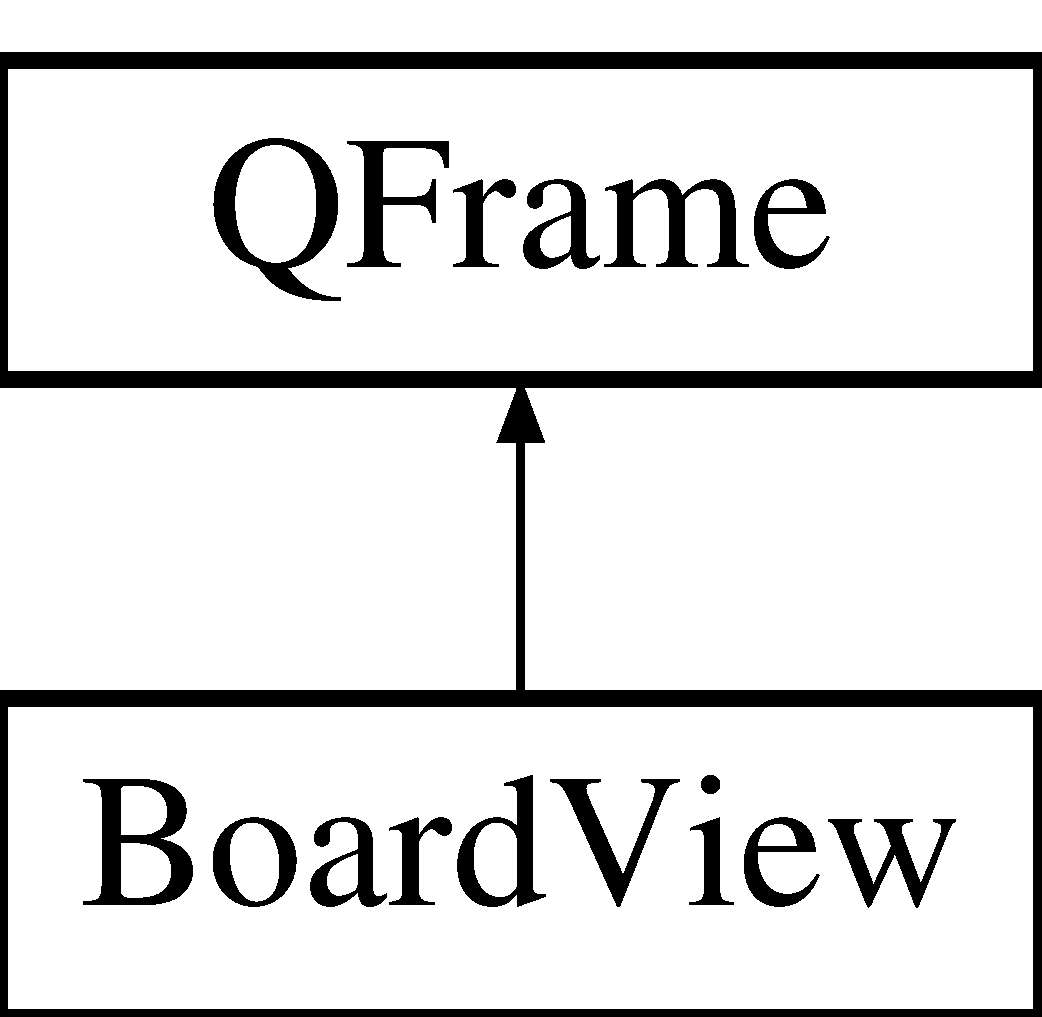
\includegraphics[height=2.000000cm]{class_board_view}
\end{center}
\end{figure}


The documentation for this class was generated from the following file\+:\begin{DoxyCompactItemize}
\item 
C\+:/\+Users/\+Olivier/\+Desktop/\+Final Tetris cleaned/\+Tetris\+\_\+\+Mikoli/boardview.\+h\end{DoxyCompactItemize}

\section{mikoli\+:\+:Buttons Class Reference}
\label{classmikoli_1_1_buttons}\index{mikoli\+::\+Buttons@{mikoli\+::\+Buttons}}


The \doxyref{Buttons}{p.}{classmikoli_1_1_buttons} class.  




{\ttfamily \#include $<$buttons.\+h$>$}

\subsection*{Public Member Functions}
\begin{DoxyCompactItemize}
\item 
\mbox{\label{classmikoli_1_1_buttons_a5676e40692022510932e31c7519f450f}} 
\textbf{ Buttons} ()
\begin{DoxyCompactList}\small\item\em \doxyref{Buttons}{p.}{classmikoli_1_1_buttons}\textquotesingle{}s constructor without parameters. This constructor uses the constructor with parameters by setting the height to 20 and the width to 10. \end{DoxyCompactList}\item 
\textbf{ Buttons} (Q\+Widget \&fenetre)
\begin{DoxyCompactList}\small\item\em \doxyref{Buttons}{p.}{classmikoli_1_1_buttons}\textquotesingle{}s constructor with Q\+Widget as parameter. This constructor is used to create a Q\+Push\+Button for the \char`\"{}\+Quick Game\char`\"{}. \end{DoxyCompactList}\item 
\textbf{ Buttons} (Q\+Widget \&fenetre, int x, int y, int width, int height, const Q\+String title)
\begin{DoxyCompactList}\small\item\em \doxyref{Buttons}{p.}{classmikoli_1_1_buttons}\textquotesingle{}s constructor with parameters. This constructor is used to create a \doxyref{Buttons}{p.}{classmikoli_1_1_buttons} configured. \end{DoxyCompactList}\item 
void \textbf{ set\+Visibility} (bool visibility)
\begin{DoxyCompactList}\small\item\em To set the visibility of the Q\+Push\+Button. \end{DoxyCompactList}\item 
\mbox{\label{classmikoli_1_1_buttons_ae4a20851f68877806fdd399af0063f10}} 
Q\+Push\+Button $\ast$ \textbf{ get\+Button} ()
\begin{DoxyCompactList}\small\item\em To get the Q\+Push\+Button. \end{DoxyCompactList}\end{DoxyCompactItemize}


\subsection{Detailed Description}
The \doxyref{Buttons}{p.}{classmikoli_1_1_buttons} class. 

This class construct an Object that contains a Q\+Push\+Buttons configured 

\subsection{Constructor \& Destructor Documentation}
\mbox{\label{classmikoli_1_1_buttons_ac51f774d8d22bfe1fd2e89e2eec30284}} 
\index{mikoli\+::\+Buttons@{mikoli\+::\+Buttons}!Buttons@{Buttons}}
\index{Buttons@{Buttons}!mikoli\+::\+Buttons@{mikoli\+::\+Buttons}}
\subsubsection{Buttons()\hspace{0.1cm}{\footnotesize\ttfamily [1/2]}}
{\footnotesize\ttfamily mikoli\+::\+Buttons\+::\+Buttons (\begin{DoxyParamCaption}\item[{Q\+Widget \&}]{fenetre }\end{DoxyParamCaption})}



\doxyref{Buttons}{p.}{classmikoli_1_1_buttons}\textquotesingle{}s constructor with Q\+Widget as parameter. This constructor is used to create a Q\+Push\+Button for the \char`\"{}\+Quick Game\char`\"{}. 


\begin{DoxyParams}{Parameters}
{\em fenetre} & the \doxyref{Widget}{p.}{class_widget} in which the Button has to appear \\
\hline
\end{DoxyParams}
\mbox{\label{classmikoli_1_1_buttons_a9314f7564a0504e19eebcdb295d68ba2}} 
\index{mikoli\+::\+Buttons@{mikoli\+::\+Buttons}!Buttons@{Buttons}}
\index{Buttons@{Buttons}!mikoli\+::\+Buttons@{mikoli\+::\+Buttons}}
\subsubsection{Buttons()\hspace{0.1cm}{\footnotesize\ttfamily [2/2]}}
{\footnotesize\ttfamily mikoli\+::\+Buttons\+::\+Buttons (\begin{DoxyParamCaption}\item[{Q\+Widget \&}]{fenetre,  }\item[{int}]{x,  }\item[{int}]{y,  }\item[{int}]{width,  }\item[{int}]{height,  }\item[{const Q\+String}]{title }\end{DoxyParamCaption})}



\doxyref{Buttons}{p.}{classmikoli_1_1_buttons}\textquotesingle{}s constructor with parameters. This constructor is used to create a \doxyref{Buttons}{p.}{classmikoli_1_1_buttons} configured. 


\begin{DoxyParams}{Parameters}
{\em fenetre} & the \doxyref{Widget}{p.}{class_widget} in which the Button has to appear \\
\hline
{\em x} & the x coordonate of the Q\+Push\+Button \\
\hline
{\em y} & the y coordonate of the Q\+Push\+Button \\
\hline
{\em width} & the Q\+Push\+Button\textquotesingle{}s with \\
\hline
{\em height} & the Q\+Push\+Button\textquotesingle{}s height \\
\hline
{\em title} & the Q\+Push\+Button\textquotesingle{}s label \\
\hline
\end{DoxyParams}


\subsection{Member Function Documentation}
\mbox{\label{classmikoli_1_1_buttons_a58dc16356e557a64078756938f37824c}} 
\index{mikoli\+::\+Buttons@{mikoli\+::\+Butto
\section{mikoli\+:\+:Choice\+Board Class Reference}
\label{classmikoli_1_1_choice_board}\index{mikoli\+::\+Choice\+Board@{mikoli\+::\+Choice\+Board}}
Inheritance diagram for mikoli\+:\+:Choice\+Board\+:\begin{figure}[H]
\begin{center}
\leavevmode
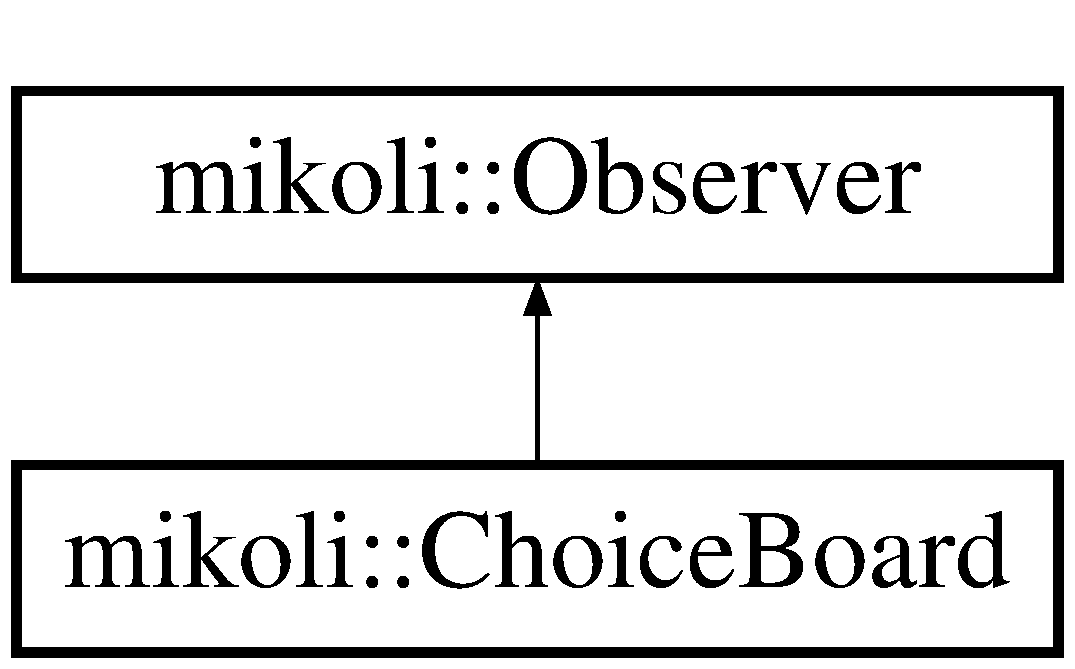
\includegraphics[height=2.000000cm]{classmikoli_1_1_choice_board}
\end{center}
\end{figure}
\subsection*{Public Member Functions}
\begin{DoxyCompactItemize}
\item 
\mbox{\label{classmikoli_1_1_choice_board_a56cea9d6275cc1669d25692de548b3f1}} 
\textbf{ Choice\+Board} ()
\begin{DoxyCompactList}\small\item\em The constructor of \doxyref{Choice\+Board}{p.}{classmikoli_1_1_choice_board} without parameters. \end{DoxyCompactList}\item 
\textbf{ Choice\+Board} (Q\+Widget \&fenetre, \textbf{ Tetris\+Game} \&game)
\begin{DoxyCompactList}\small\item\em The constructor of \doxyref{Choice\+Board}{p.}{classmikoli_1_1_choice_board} with parameters. \end{DoxyCompactList}\item 
\mbox{\label{classmikoli_1_1_choice_board_a96fcebaacc4ba180542a472b898633a6}} 
Gamemode \textbf{ get\+Mode} ()
\begin{DoxyCompactList}\small\item\em To get the Game\+Mode. \end{DoxyCompactList}\item 
\mbox{\label{classmikoli_1_1_choice_board_a8e819e30d9da07531725f36c5537b09b}} 
Q\+Push\+Button $\ast$ \textbf{ get\+Button\+Restart} ()
\begin{DoxyCompactList}\small\item\em To get the restart Button. \end{DoxyCompactList}\item 
\mbox{\label{classmikoli_1_1_choice_board_aa29d3048e930a7f9fa18577608055e9c}} 
Q\+Push\+Button $\ast$ \textbf{ get\+Button\+New\+Game} ()
\begin{DoxyCompactList}\small\item\em To get the New\+Game Button. \end{DoxyCompactList}\item 
\mbox{\label{classmikoli_1_1_choice_board_a99deeabe045b9f035795e580bc26ddb4}} 
Q\+Push\+Button $\ast$ \textbf{ get\+Button\+Quick\+Game} ()
\begin{DoxyCompactList}\small\item\em To get the Quick\+Game Button. \end{DoxyCompactList}\item 
int \textbf{ get\+Mode\+Value} (Gamemode mode)
\begin{DoxyCompactList}\small\item\em To get the Game mode value (which is the goal) \end{DoxyCompactList}\item 
\mbox{\label{classmikoli_1_1_choice_board_a9b5fd6e4d9b26eb3dd34e358c264ee87}} 
void \textbf{ hide} ()
\begin{DoxyCompactList}\small\item\em To hide the \doxyref{Choice\+Board}{p.}{classmikoli_1_1_choice_board}. \end{DoxyCompactList}\item 
\mbox{\label{classmikoli_1_1_choice_board_a49670195ba61639711c25fb4b0f4fce4}} 
void \textbf{ show} ()
\begin{DoxyCompactList}\small\item\em To show the \doxyref{Choice\+Board}{p.}{classmikoli_1_1_choice_board} with the \doxyref{Buttons}{p.}{classmikoli_1_1_buttons}. \end{DoxyCompactList}\item 
\mbox{\label{classmikoli_1_1_choice_board_a2a60a41bfb3657b37debd4446ef319aa}} 
void \textbf{ show\+Choose\+Menu} ()
\begin{DoxyCompactList}\small\item\em To show the \doxyref{Choice\+Board}{p.}{classmikoli_1_1_choice_board} (only the radiobuttons and spin boxes) \end{DoxyCompactList}\item 
\mbox{\label{classmikoli_1_1_choice_board_a5bceb67d36d1b5090908037280cf4eb6}} 
void \textbf{ Update} ()
\begin{DoxyCompactList}\small\item\em The method executed when the observable changed. \end{DoxyCompactList}\end{DoxyCompactItemize}
\subsection*{Additional Inherited Members}


\subsection{Constructor \& Destructor Documentation}
\mbox{\label{classmikoli_1_1_choice_board_ab3828086b7eea78e87be1c3b5af03c62}} 
\index{mikoli\+::\+Choice\+Board@{mikoli\+::\+Choice\+Board}!Choice\+Board@{Choice\+Board}}
\index{Choice\+Board@{Choice\+Board}!mikoli\+::\+Choice\+Board@{mikoli\+::\+Choice\+Board}}
\subsubsection{Choice\+Board()}
{\footnotesize\ttfamily mikoli\+::\+Choice\+Board\+::\+Choice\+Board (\begin{DoxyParamCaption}\item[{Q\+Widget \&}]{fenetre,  }\item[{\textbf{ Tetris\+Game} \&}]{game }\end{DoxyParamCaption})}



The constructor of \doxyref{Choice\+Board}{p.}{classmikoli_1_1_choice_board} with parameters. 


\begin{DoxyParams}{Parameters}
{\em fenetre} & the \doxyref{Widget}{p.}{class_widget} in which the \doxyref{Choice\+Board}{p.}{classmikoli_1_1_choice_board} has to appear \\
\hline
{\em game} & the \doxyref{Tetris\+Game}{p.}{classmikoli_1_1_tetris_game} \\
\hline
\end{DoxyParams}


\subsection{Member Function Documentation}
\mbox{\label{classmikoli_1_1_choice_board_ad814e9257e9ae6f65710a9855c66527c}} 
\index{mikoli\+::\+Choice\+Board@{mikoli\+::\+Choice\+Board}!get\+Mode\+Value@{get\+Mode\+Value}}
\index{get\+Mode\+Value@{get\+Mode\+Value}!mikoli\+::\+Choice\+Board@{mikoli\+::\+Choice\+Board}}
\subsubsection{get\+Mode\+Value()}
{\footnotesize\ttfamily int mikoli\+::\+Choice\+Board\+::get\+Mode\+Value (\begin{DoxyParamCaption}\item[{Gamemode}]{mode }\end{DoxyParamCaption})}



To get the Game mode value (which is the goal) 


\begin{DoxyParams}{Parameters}
{\em mode} & the Gamemode \\
\hline
\end{DoxyParams}


The documentation for this class was generated from the following files\+:\begin{DoxyCompactItemize}
\item 
C\+:/\+Users/\+Olivier/\+Desktop/\+Final Tetris cleaned/\+Tetris\+\_\+\+Mikoli/choiceboard.\+h\item 
C\+:/\+Users/\+Olivier/\+Desktop/\+Final Tetris cleaned/\+Tetris\+\_\+\+Mikoli/choiceboard.\+cpp\end{DoxyCompactItemize}

\section{Controller Class Reference}
\label{class_controller}\index{Controller@{Controller}}


The documentation for this class was generated from the following files\+:\begin{DoxyCompactItemize}
\item 
C\+:/\+Users/\+Olivier/\+Desktop/\+Final Tetris cleaned/\+Tetris\+\_\+\+Mikoli/controller.\+h\item 
C\+:/\+Users/\+Olivier/\+Desktop/\+Final Tetris cleaned/\+Tetris\+\_\+\+Mikoli/controller.\+cpp\end{DoxyCompactItemize}

\section{mikoli\+:\+:Figure Class Reference}
\label{classmikoli_1_1_figure}\index{mikoli\+::\+Figure@{mikoli\+::\+Figure}}


The \doxyref{Figure}{p.}{classmikoli_1_1_figure} class.  




{\ttfamily \#include $<$figure.\+h$>$}

\subsection*{Public Member Functions}
\begin{DoxyCompactItemize}
\item 
\mbox{\label{classmikoli_1_1_figure_af48a1d65138534359444f46ff2cac139}} 
\textbf{ Figure} ()
\begin{DoxyCompactList}\small\item\em Figures constructor without parameters. This constructor will use the constructor without parameters og \doxyref{Position}{p.}{classmikoli_1_1_position} for initializing the attribute \+\_\+position and settings the \+\_\+color attribute to red. \end{DoxyCompactList}\item 
\textbf{ Figure} (Type\+Shape type\+Shape)
\begin{DoxyCompactList}\small\item\em Figures Constructor with parameters. \end{DoxyCompactList}\item 
\mbox{\label{classmikoli_1_1_figure_af851763ba4fb93940ad0584647d5028d}} 
\textbf{ $\sim$\+Figure} ()
\begin{DoxyCompactList}\small\item\em Figures destructor. \end{DoxyCompactList}\item 
std\+::vector$<$ \textbf{ Position} $>$ \textbf{ get\+Positions} ()
\begin{DoxyCompactList}\small\item\em get\+Positions \end{DoxyCompactList}\item 
std\+::vector$<$ \textbf{ Block} $>$ \textbf{ get\+Blocks} ()
\begin{DoxyCompactList}\small\item\em get\+Blocks \end{DoxyCompactList}\item 
Type\+Shape \textbf{ get\+Type\+Figure} ()
\begin{DoxyCompactList}\small\item\em get\+Type\+Figure \end{DoxyCompactList}\item 
\mbox{\label{classmikoli_1_1_figure_a2b86d8f2178edbf39f4a9d4312e3f880}} 
void {\bfseries set\+Blocks} (std\+::vector$<$ \textbf{ Block} $>$)
\item 
void \textbf{ move} (Direction direction)
\begin{DoxyCompactList}\small\item\em move Makes it possible to move a figure to the left, right or down. \end{DoxyCompactList}\item 
void \textbf{ rotate} (Direction direction)
\begin{DoxyCompactList}\small\item\em rotate Makes it possible to rotate a figure to the left or to the right. \end{DoxyCompactList}\item 
void \textbf{ new\+Position} (\textbf{ Position} position)
\begin{DoxyCompactList}\small\item\em new\+Position Makes it possible to displace a figure by modifying the location of its central point. \end{DoxyCompactList}\end{DoxyCompactItemize}


\subsection{Detailed Description}
The \doxyref{Figure}{p.}{classmikoli_1_1_figure} class. 

This class is used to construct a figure. A figure is composed with 4 blocks and a center point around which the figure can rotate. \+\_\+\+Blocks An array of 4 blocks . \+\_\+axe\+Point The point around which the figure can rotate also used to put a figure in the board at a certain position. 

\subsection{Constructor \& Destructor Documentation}
\mbox{\label{classmikoli_1_1_figure_a5c6b4df3de6ddb6a36a2d86501fbe311}} 
\index{mikoli\+::\+Figure@{mikoli\+::\+Figure}!Figure@{Figure}}
\index{Figure@{Figure}!mikoli\+::\+Figure@{mikoli\+::\+Figure}}
\subsubsection{Figure()}
{\footnotesize\ttfamily mikoli\+::\+Figure\+::\+Figure (\begin{DoxyParamCaption}\item[{Type\+Shape}]{type\+Shape }\end{DoxyParamCaption})}



Figures Constructor with parameters. 


\begin{DoxyParams}{Parameters}
{\em type\+Shape} & The type of the \doxyref{Figure}{p.}{classmikoli_1_1_figure}. \\
\hline
\end{DoxyParams}


\subsection{Member Function Documentation}
\mbox{\label{classmikoli_1_1_figure_a07bfd00b5da770802438a75a79a76084}} 
\index{mikoli\+::\+Figure@{mikoli\+::\+Figure}!get\+Blocks@{get\+Blocks}}
\index{get\+Blocks@{get\+Blocks}!mikoli\+::\+Figure@{mikoli\+::\+Figure}}
\subsubsection{get\+Blocks()}
{\footnotesize\ttfamily std\+::vector$<$ \textbf{ Block} $>$ mikoli\+::\+Figure\+::get\+Blocks (\begin{DoxyParamCaption}{ }\end{DoxyParamCaption})}



get\+Blocks 

\begin{DoxyReturn}{Returns}
return a list of Blocks which forms the figure. 
\end{DoxyReturn}
\mbox{\label{classmikoli_1_1_figure_a996d2b91660d2b8cdd989f7e3a128661}} 
\index{mikoli\+::\+Figure@{mikoli\+::\+Figure}!get\+Positions@{get\+Positions}}
\index{get\+Positions@{get\+Positions}!mikoli\+::\+Figure@{mikoli\+::\+Figure}}
\subsubsection{get\+Positions()}
{\footnotesize\ttfamily std\+::vector$<$ \textbf{ Position} $>$ mikoli\+::\+Figu
\section{mikoli\+:\+:Figures\+Bag Class Reference}
\label{classmikoli_1_1_figures_bag}\index{mikoli\+::\+Figures\+Bag@{mikoli\+::\+Figures\+Bag}}


The \doxyref{Figures\+Bag}{p.}{classmikoli_1_1_figures_bag} class.  




{\ttfamily \#include $<$figuresbag.\+h$>$}

\subsection*{Public Member Functions}
\begin{DoxyCompactItemize}
\item 
\mbox{\label{classmikoli_1_1_figures_bag_a3fab8cb8bc3a9932fc4ceaa67efe56eb}} 
\textbf{ Figures\+Bag} ()
\begin{DoxyCompactList}\small\item\em \doxyref{Figures\+Bag}{p.}{classmikoli_1_1_figures_bag} constructor without parameters. This constructor will initialize the \doxyref{Figures\+Bag}{p.}{classmikoli_1_1_figures_bag} with default parameters. \end{DoxyCompactList}\item 
\mbox{\label{classmikoli_1_1_figures_bag_a6a167b920ebadf48639fe2c7ad8bdcbb}} 
\textbf{ $\sim$\+Figures\+Bag} ()
\begin{DoxyCompactList}\small\item\em \doxyref{Figures\+Bag}{p.}{classmikoli_1_1_figures_bag} destructor. Deallocate the memory that was previously reserved for the \doxyref{Figures\+Bag}{p.}{classmikoli_1_1_figures_bag}. \end{DoxyCompactList}\item 
\textbf{ Figure} \textbf{ get\+Next\+Figure} ()
\begin{DoxyCompactList}\small\item\em get\+Type() Recover the type of the figure \end{DoxyCompactList}\item 
\mbox{\label{classmikoli_1_1_figures_bag_a415c54519dae9e094936c11558c1c9f2}} 
void \textbf{ refresh} ()
\begin{DoxyCompactList}\small\item\em refresh Reinitialize the \doxyref{Figures\+Bag}{p.}{classmikoli_1_1_figures_bag} when the \doxyref{Figures\+Bag}{p.}{classmikoli_1_1_figures_bag} is empty. \end{DoxyCompactList}\end{DoxyCompactItemize}


\subsection{Detailed Description}
The \doxyref{Figures\+Bag}{p.}{classmikoli_1_1_figures_bag} class. 

\+\_\+next\+Figure The \doxyref{Figure}{p.}{classmikoli_1_1_figure} that will become the current \doxyref{Figure}{p.}{classmikoli_1_1_figure}. \+\_\+list\+Figures The list of differents figures that will be played. 

\subsection{Member Function Documentation}
\mbox{\label{classmikoli_1_1_figures_bag_aa4db3d3c59fbb2d5aba2081d05d0787f}} 
\index{mikoli\+::\+Figures\+Bag@{mikoli\+::\+Figures\+Bag}!get\+Next\+Figure@{get\+Next\+Figure}}
\index{get\+Next\+Figure@{get\+Next\+Figure}!mikoli\+::\+Figures\+Bag@{mikoli\+::\+Figures\+Bag}}
\subsubsection{get\+Next\+Figure()}
{\footnotesize\ttfamily \textbf{ Figure} mikoli\+::\+Figures\+Bag\+::get\+Next\+Figure (\begin{DoxyParamCaption}{ }\end{DoxyParamCaption})}



get\+Type() Recover the type of the figure 

\begin{DoxyReturn}{Returns}
The next \doxyref{Figure}{p.}{classmikoli_1_1_figure} that will become the current \doxyref{Figure}{p.}{classmikoli_1_1_figure}. 
\end{DoxyReturn}


The documentation for this class was generated from the following files\+:\begin{DoxyCompactItemize}
\item 
C\+:/\+Users/\+Olivier/\+Desktop/\+Final Tetris cleaned/\+Tetris\+\_\+\+Mikoli/figuresbag.\+h\item 
C\+:/\+Users/\+Olivier/\+Desktop/\+Final Tetris cleaned/\+Tetris\+\_\+\+Mikoli/figuresbag.\+cpp\end{DoxyCompactItemize}

\section{mikoli\+:\+:Main\+Control Class Reference}
\label{classmikoli_1_1_main_control}\index{mikoli\+::\+Main\+Control@{mikoli\+::\+Main\+Control}}


The \doxyref{Main\+Control}{p.}{classmikoli_1_1_main_control} class This class is the controller of the game. It is the interface between the G\+UI and the model. It receives the informations from the user and call the methods necessary. It will start the game.  




{\ttfamily \#include $<$maincontrol.\+h$>$}

\subsection*{Public Member Functions}
\begin{DoxyCompactItemize}
\item 
\mbox{\label{classmikoli_1_1_main_control_a064bf042117c6359584b4dc49924dcec}} 
void \textbf{ start\+New\+Game} ()
\begin{DoxyCompactList}\small\item\em start\+New\+Game It create a new game with standard options \end{DoxyCompactList}\item 
\mbox{\label{classmikoli_1_1_main_control_a4ba6b36bce217d667ef953927edea9d8}} 
void \textbf{ select\+Mode} (Game\+Mode game\+Mode)
\begin{DoxyCompactList}\small\item\em select\+Mode It makes possible to choose differents game mode. \end{DoxyCompactList}\item 
\mbox{\label{classmikoli_1_1_main_control_af212f7f8dbce2ff10a14336e62256c5c}} 
void \textbf{ customize} ()
\begin{DoxyCompactList}\small\item\em customize It makes possible to create cusztomized Figures that could be added to the game \end{DoxyCompactList}\item 
\mbox{\label{classmikoli_1_1_main_control_a3f48c4101c4655217b5136ece6c692ed}} 
void \textbf{ exit\+App} ()
\begin{DoxyCompactList}\small\item\em exit\+App Method that closes the application. \end{DoxyCompactList}\end{DoxyCompactItemize}


\subsection{Detailed Description}
The \doxyref{Main\+Control}{p.}{classmikoli_1_1_main_control} class This class is the controller of the game. It is the interface between the G\+UI and the model. It receives the informations from the user and call the methods necessary. It will start the game. 

The documentation for this class was generated from the following file\+:\begin{DoxyCompactItemize}
\item 
C\+:/\+Users/\+Olivier/\+Desktop/\+Final Tetris cleaned/\+Tetris\+\_\+\+Mikoli/maincontrol.\+h\end{DoxyCompactItemize}

\section{mikoli\+:\+:Mode Class Reference}
\label{classmikoli_1_1_mode}\index{mikoli\+::\+Mode@{mikoli\+::\+Mode}}


The \doxyref{Mode}{p.}{classmikoli_1_1_mode} class Manage the game mode of the game. By this class, it\textquotesingle{}s possible to switch between different game modes.  




{\ttfamily \#include $<$mode.\+h$>$}

\subsection*{Public Member Functions}
\begin{DoxyCompactItemize}
\item 
\mbox{\label{classmikoli_1_1_mode_a1c3d983b4b6b187282471a6c8da12106}} 
\textbf{ Mode} ()
\begin{DoxyCompactList}\small\item\em \doxyref{Mode}{p.}{classmikoli_1_1_mode} Constructor by default. \end{DoxyCompactList}\item 
\mbox{\label{classmikoli_1_1_mode_a6118f201e1505676831fbd8849a29265}} 
\textbf{ Mode} (Gamemode, int)
\begin{DoxyCompactList}\small\item\em \doxyref{Mode}{p.}{classmikoli_1_1_mode} Constructor with parameters. Gamemode is the game mode of the game. int is the goal to reach. \end{DoxyCompactList}\item 
Gamemode \textbf{ get\+Game\+Mode} ()
\begin{DoxyCompactList}\small\item\em get\+Game\+Mode \end{DoxyCompactList}\item 
int \textbf{ get\+Goal} ()
\begin{DoxyCompactList}\small\item\em get\+Goal \end{DoxyCompactList}\item 
\mbox{\label{classmikoli_1_1_mode_ae9c08d8cb4af815806412fdcab4d16a1}} 
void \textbf{ set\+Game\+Mode} (Gamemode)
\begin{DoxyCompactList}\small\item\em set\+Game\+Mode Set a new game mode to the game. \end{DoxyCompactList}\item 
\mbox{\label{classmikoli_1_1_mode_ac29f131a55659d8d3cf3b0493c0f15f3}} 
void \textbf{ set\+Goal} (int)
\begin{DoxyCompactList}\small\item\em set\+Goal Set a new goal to reach. \end{DoxyCompactList}\end{DoxyCompactItemize}


\subsection{Detailed Description}
The \doxyref{Mode}{p.}{classmikoli_1_1_mode} class Manage the game mode of the game. By this class, it\textquotesingle{}s possible to switch between different game modes. 

\subsection{Member Function Documentation}
\mbox{\label{classmikoli_1_1_mode_aa77e745b210f6afa85fc6a1cceed4815}} 
\index{mikoli\+::\+Mode@{mikoli\+::\+Mode}!get\+Game\+Mode@{get\+Game\+Mode}}
\index{get\+Game\+Mode@{get\+Game\+Mode}!mikoli\+::\+Mode@{mikoli\+::\+Mode}}
\subsubsection{get\+Game\+Mode()}
{\footnotesize\ttfamily Gamemode mikoli\+::\+Mode\+::get\+Game\+Mode (\begin{DoxyParamCaption}{ }\end{DoxyParamCaption})}



get\+Game\+Mode 

\begin{DoxyReturn}{Returns}
The current game mode of the game. 
\end{DoxyReturn}
\mbox{\label{classmikoli_1_1_mode_a08172c542b67e26c680f994b61532bbe}} 
\index{mikoli\+::\+Mode@{mikoli\+::\+Mode}!get\+Goal@{get\+Goal}}
\index{get\+Goal@{get\+Goal}!mikoli\+::\+Mode@{mikoli\+::\+Mode}}
\subsubsection{get\+Goal()}
{\footnotesize\ttfamily int mikoli\+::\+Mode\+::get\+Goal (\begin{DoxyParamCaption}{ }\end{DoxyParamCaption})}



get\+Goal 

\begin{DoxyReturn}{Returns}
The goal to reach. 
\end{DoxyReturn}


The documentation for this class was generated from the following files\+:\begin{DoxyCompactItemize}
\item 
C\+:/\+Users/\+Olivier/\+Desktop/\+Final Tetris cleaned/\+Tetris\+\_\+\+Mikoli/mode.\+h\item 
C\+:/\+Users/\+Olivier/\+Desktop/\+Final Tetris cleaned/\+Tetris\+\_\+\+Mikoli/mode.\+cpp\end{DoxyCompactItemize}

\section{My\+Lcd Class Reference}
\label{class_my_lcd}\index{My\+Lcd@{My\+Lcd}}
Inheritance diagram for My\+Lcd\+:\begin{figure}[H]
\begin{center}
\leavevmode
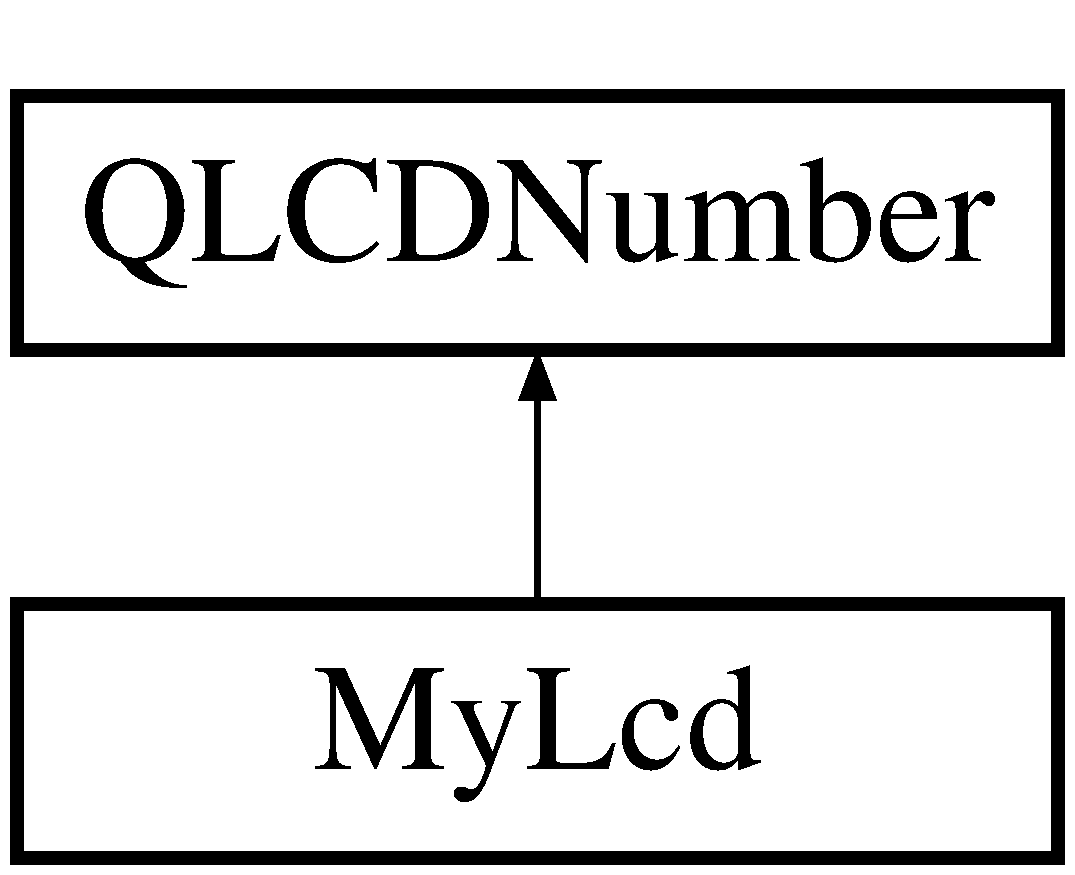
\includegraphics[height=2.000000cm]{class_my_lcd}
\end{center}
\end{figure}
\subsection*{Public Member Functions}
\begin{DoxyCompactItemize}
\item 
\mbox{\label{class_my_lcd_a166dd1e079205d4c4c2693e1b0c054b4}} 
{\bfseries My\+Lcd} (int value)
\item 
\mbox{\label{class_my_lcd_a43dce43e1ce2fb161e08041532eba134}} 
void {\bfseries set\+Value} (int value)
\end{DoxyCompactItemize}


The documentation for this class was generated from the following files\+:\begin{DoxyCompactItemize}
\item 
C\+:/\+Users/\+Olivier/\+Desktop/\+Final Tetris cleaned/\+Tetris\+\_\+\+Mikoli/mylcd.\+h\item 
C\+:/\+Users/\+Olivier/\+Desktop/\+Final Tetris cleaned/\+Tetris\+\_\+\+Mikoli/mylcd.\+cpp\end{DoxyCompactItemize}

\section{mikoli\+:\+:Observable Class Reference}
\label{classmikoli_1_1_observable}\index{mikoli\+::\+Observable@{mikoli\+::\+Observable}}


The \doxyref{Observable}{p.}{classmikoli_1_1_observable} class Interface implemented by the classes that have to be observed.  




{\ttfamily \#include $<$observable.\+h$>$}

Inheritance diagram for mikoli\+:\+:Observable\+:\begin{figure}[H]
\begin{center}
\leavevmode
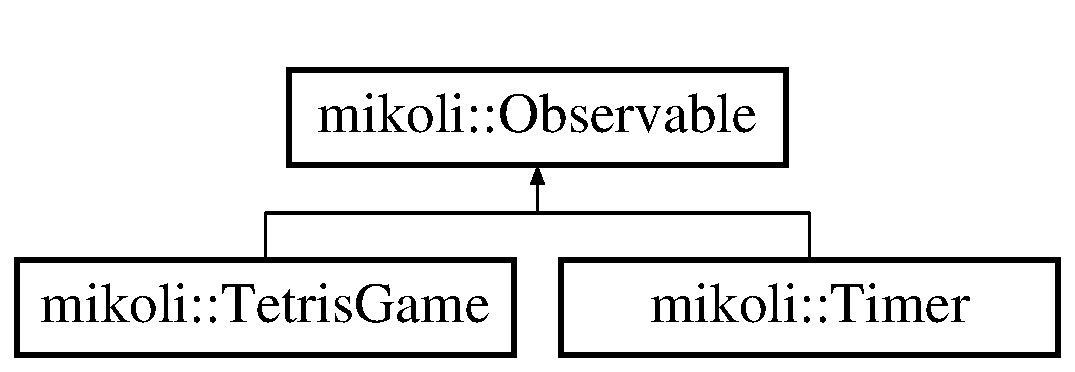
\includegraphics[height=2.000000cm]{classmikoli_1_1_observable}
\end{center}
\end{figure}
\subsection*{Public Member Functions}
\begin{DoxyCompactItemize}
\item 
\mbox{\label{classmikoli_1_1_observable_aa914d67b64d23d3dda3bb8b73f351ec0}} 
void {\bfseries Add\+Obs} (\textbf{ Observer} $\ast$obs)
\item 
\mbox{\label{classmikoli_1_1_observable_a63215bec5261ec6f89240013e435e3f7}} 
void {\bfseries Del\+Obs} (\textbf{ Observer} $\ast$obs)
\item 
\mbox{\label{classmikoli_1_1_observable_a5bb6e044f5927c7025d57e5a35851e8a}} 
void {\bfseries Notify} (void)
\end{DoxyCompactItemize}


\subsection{Detailed Description}
The \doxyref{Observable}{p.}{classmikoli_1_1_observable} class Interface implemented by the classes that have to be observed. 

The documentation for this class was generated from the following files\+:\begin{DoxyCompactItemize}
\item 
C\+:/\+Users/\+Olivier/\+Desktop/\+Final Tetris cleaned/\+Tetris\+\_\+\+Mikoli/observable.\+h\item 
C\+:/\+Users/\+Olivier/\+Desktop/\+Final Tetris cleaned/\+Tetris\+\_\+\+Mikoli/observable.\+cpp\end{DoxyCompactItemize}

\section{mikoli\+:\+:Observer Class Reference}
\label{classmikoli_1_1_observer}\index{mikoli\+::\+Observer@{mikoli\+::\+Observer}}


The \doxyref{Observer}{p.}{classmikoli_1_1_observer} class Implemented by the class that have to Observe another class(observable)  




{\ttfamily \#include $<$observer.\+h$>$}

Inheritance diagram for mikoli\+:\+:Observer\+:\begin{figure}[H]
\begin{center}
\leavevmode
\includegraphics[height=1.709924cm]{classmikoli_1_1_observer}
\end{center}
\end{figure}
\subsection*{Public Member Functions}
\begin{DoxyCompactItemize}
\item 
\mbox{\label{classmikoli_1_1_observer_a5492a5fc3f7e81ec7bd9bbdb81614f21}} 
virtual void {\bfseries Update} ()=0
\item 
\mbox{\label{classmikoli_1_1_observer_a1c24a11256659f80c6956274808100c4}} 
void {\bfseries Add\+Obs} (\textbf{ Observable} $\ast$obs)
\item 
\mbox{\label{classmikoli_1_1_observer_a02036eb909a2a08b0ca5dc5485c81162}} 
void {\bfseries Del\+Obs} (\textbf{ Observable} $\ast$obs)
\end{DoxyCompactItemize}
\subsection*{Protected Types}
\begin{DoxyCompactItemize}
\item 
\mbox{\label{classmikoli_1_1_observer_a92209a844c15655dc0bdec717756e0f2}} 
typedef std\+::list$<$ \textbf{ Observable} $\ast$ $>$\+::iterator {\bfseries iterator}
\item 
\mbox{\label{classmikoli_1_1_observer_a06f08c18caa6931b3b5e1d38a3e5541a}} 
typedef std\+::list$<$ \textbf{ Observable} $\ast$ $>$\+::const\+\_\+iterator {\bfseries const\+\_\+iterator}
\end{DoxyCompactItemize}
\subsection*{Protected Attributes}
\begin{DoxyCompactItemize}
\item 
\mbox{\label{classmikoli_1_1_observer_a2fa3a68b9a98dc6469807f80d0e1e4f1}} 
std\+::list$<$ \textbf{ Observable} $\ast$ $>$ {\bfseries m\+\_\+list}
\end{DoxyCompactItemize}


\subsection{Detailed Description}
The \doxyref{Observer}{p.}{classmikoli_1_1_observer} class Implemented by the class that have to Observe another class(observable) 

The documentation for this class was generated from the following files\+:\begin{DoxyCompactItemize}
\item 
C\+:/\+Users/\+Olivier/\+Desktop/\+Final Tetris cleaned/\+Tetris\+\_\+\+Mikoli/observer.\+h\item 
C\+:/\+Users/\+Olivier/\+Desktop/\+Final Tetris cleaned/\+Tetris\+\_\+\+Mikoli/observer.\+cpp\end{DoxyCompactItemize}

\section{mikoli\+:\+:Paint\+Board Class Reference}
\label{classmikoli_1_1_paint_board}\index{mikoli\+::\+Paint\+Board@{mikoli\+::\+Paint\+Board}}
Inheritance diagram for mikoli\+:\+:Paint\+Board\+:\begin{figure}[H]
\begin{center}
\leavevmode
\includegraphics[height=2.000000cm]{classmikoli_1_1_paint_board}
\end{center}
\end{figure}
\subsection*{Public Member Functions}
\begin{DoxyCompactItemize}
\item 
\mbox{\label{classmikoli_1_1_paint_board_ad976d76f5064307ea77373e107d6424c}} 
{\bfseries Paint\+Board} (Q\+Widget \&fenetre, \textbf{ Tetris\+Game} \&game)
\item 
\mbox{\label{classmikoli_1_1_paint_board_a6ab43b112e7302f435a1ded710c9dcab}} 
void {\bfseries Update} (const \textbf{ Observable} $\ast$observable)
\end{DoxyCompactItemize}
\subsection*{Protected Member Functions}
\begin{DoxyCompactItemize}
\item 
\mbox{\label{classmikoli_1_1_paint_board_a6ac5cefd98cf2111ef231f842319948c}} 
void {\bfseries paint\+Event} (Q\+Widget \&fenetre, Q\+Paint\+Event $\ast$event)
\end{DoxyCompactItemize}
\subsection*{Additional Inherited Members}


The documentation for this class was generated from the following files\+:\begin{DoxyCompactItemize}
\item 
C\+:/\+Users/\+Olivier/\+Desktop/\+Final Tetris cleaned/\+Tetris\+\_\+\+Mikoli/paintboard.\+h\item 
C\+:/\+Users/\+Olivier/\+Desktop/\+Final Tetris cleaned/\+Tetris\+\_\+\+Mikoli/paintboard.\+cpp\end{DoxyCompactItemize}

\section{mikoli\+:\+:Position Class Reference}
\label{classmikoli_1_1_position}\index{mikoli\+::\+Position@{mikoli\+::\+Position}}


The \doxyref{Position}{p.}{classmikoli_1_1_position} class.  




{\ttfamily \#include $<$position.\+h$>$}

\subsection*{Public Member Functions}
\begin{DoxyCompactItemize}
\item 
\mbox{\label{classmikoli_1_1_position_a885fea7b7c57c74996ce83a2bc3c476b}} 
\textbf{ Position} ()
\begin{DoxyCompactList}\small\item\em \doxyref{Position}{p.}{classmikoli_1_1_position}\textquotesingle{}s constructor without parameters. This constructor will set the \+\_\+x attribute and Y to 0. \end{DoxyCompactList}\item 
\textbf{ Position} (int x, int y)
\begin{DoxyCompactList}\small\item\em \doxyref{Position}{p.}{classmikoli_1_1_position}\textquotesingle{}s constructor with 2 parameters. \end{DoxyCompactList}\item 
\mbox{\label{classmikoli_1_1_position_a376c221beb59a3ac86c749c661e94f0e}} 
\textbf{ $\sim$\+Position} ()
\begin{DoxyCompactList}\small\item\em \doxyref{Position}{p.}{classmikoli_1_1_position}\textquotesingle{}s destructor. \end{DoxyCompactList}\item 
int \textbf{ getX} ()
\begin{DoxyCompactList}\small\item\em getX \end{DoxyCompactList}\item 
int \textbf{ getY} ()
\begin{DoxyCompactList}\small\item\em getY \end{DoxyCompactList}\item 
void \textbf{ setX} (int x)
\begin{DoxyCompactList}\small\item\em setX \end{DoxyCompactList}\item 
void \textbf{ setY} (int y)
\begin{DoxyCompactList}\small\item\em setY \end{DoxyCompactList}\item 
bool \textbf{ is\+Same} (\textbf{ Position} position)
\begin{DoxyCompactList}\small\item\em is\+Same \end{DoxyCompactList}\end{DoxyCompactItemize}


\subsection{Detailed Description}
The \doxyref{Position}{p.}{classmikoli_1_1_position} class. 

This class will be used to determinate the \doxyref{Block}{p.}{classmikoli_1_1_block}\textquotesingle{}s \doxyref{Position}{p.}{classmikoli_1_1_position} in the board. \+\_\+x The abscissa. \+\_\+y The ordinate. 

\subsection{Constructor \& Destructor Documentation}
\mbox{\label{classmikoli_1_1_position_a32a684df59f7be1fe1e1844930d68a77}} 
\index{mikoli\+::\+Position@{mikoli\+::\+Position}!Position@{Position}}
\index{Position@{Position}!mikoli\+::\+Position@{mikoli\+::\+Position}}
\subsubsection{Position()}
{\footnotesize\ttfamily mikoli\+::\+Position\+::\+Position (\begin{DoxyParamCaption}\item[{int}]{x,  }\item[{int}]{y }\end{DoxyParamCaption})}



\doxyref{Position}{p.}{classmikoli_1_1_position}\textquotesingle{}s constructor with 2 parameters. 


\begin{DoxyParams}{Parameters}
{\em x} & the value for horizontal axis. \\
\hline
{\em y} & the value for vertical axis. \\
\hline
\end{DoxyParams}


\subsection{Member Function Documentation}
\mbox{\label{classmikoli_1_1_position_a0176c944297a742b30a1197b336c9ac2}} 
\index{mikoli\+::\+Position@{mikoli\+::\+Position}!getX@{getX}}
\index{getX@{getX}!mikoli\+::\+Position@{mikoli\+::\+Position}}
\subsubsection{get\+X()}
{\footnotesize\ttfamily int mikoli\+::\+Position\+::getX (\begin{DoxyParamCaption}{ }\end{DoxyParamCaption})}



getX 

\begin{DoxyReturn}{Returns}
The value of \+\_\+x. 
\end{DoxyReturn}
\mbox{\label{classmikoli_1_1_position_abaab55b498370b71d083681cde3b2b37}} 
\index{mikoli\+::\+Position@{mikoli\+::\+Position}!getY@{getY}}
\index{getY@{getY}!mikoli\+::\+Position@{mikoli\+::\+Position}}
\subsubsection{get\+Y()}
{\footnotesize\ttfamily int mikoli\+::\+Position\+::getY (\begin{DoxyParamCaption}{ }\end{DoxyParamCaption})}



getY 

\begin{DoxyReturn}{Returns}
The value of \+\_\+y. 
\end{DoxyReturn}
\mbox{\label{classmikoli_1_1_position_af485cb080aa2f97f9cd10ca3b2e02bad}} 
\index{mikoli\+::\+Position@{mikoli\+::\+Position}!is\+Same@{is\+Same}}
\index{is\+Same@{is\+Same}!mikoli\+::\+Position@{mikoli\+::\+Position}}
\subsubsection{is\+Same()}
{\footnotesize\ttfamily bool mikoli\+::\+Position\+::is\+Same (\begin{DoxyParamCaption}\item[{\textbf{ Position}}]{position }\end{DoxyParamCaption})}



is\+Same 


\begin{DoxyParams}{Parameters}
{\em position} & The position to compare to. \\
\hline
\end{DoxyParams}
\begin{DoxyReturn}{Returns}
true if The position is the same, false otherwise. 
\
\section{qt\+\_\+meta\+\_\+stringdata\+\_\+\+Widget\+\_\+t Struct Reference}
\label{structqt__meta__stringdata___widget__t}\index{qt\+\_\+meta\+\_\+stringdata\+\_\+\+Widget\+\_\+t@{qt\+\_\+meta\+\_\+stringdata\+\_\+\+Widget\+\_\+t}}
\subsection*{Public Attributes}
\begin{DoxyCompactItemize}
\item 
\mbox{\label{structqt__meta__stringdata___widget__t_a9fe3de556b708897fb7eb999f1efbfcb}} 
Q\+Byte\+Array\+Data {\bfseries data} [1]
\item 
\mbox{\label{structqt__meta__stringdata___widget__t_abfd6a2b9daf76d6315586d12e8b7ec36}} 
char {\bfseries stringdata0} [7]
\end{DoxyCompactItemize}


The documentation for this struct was generated from the following file\+:\begin{DoxyCompactItemize}
\item 
C\+:/\+Users/\+Olivier/\+Desktop/\+Final Tetris cleaned/\+Tetris\+\_\+\+Mikoli/moc\+\_\+widget.\+cpp\end{DoxyCompactItemize}

\section{mikoli\+:\+:Score Class Reference}
\label{classmikoli_1_1_score}\index{mikoli\+::\+Score@{mikoli\+::\+Score}}


The \doxyref{Score}{p.}{classmikoli_1_1_score} class This class will inform the score of the user and the number of lines he\textquotesingle{}s done. Also used buy the G\+UI.  




{\ttfamily \#include $<$score.\+h$>$}

\subsection*{Public Member Functions}
\begin{DoxyCompactItemize}
\item 
\mbox{\label{classmikoli_1_1_score_a30609739c62d21c769fbacedb32056df}} 
\textbf{ Score} ()
\begin{DoxyCompactList}\small\item\em \doxyref{Score}{p.}{classmikoli_1_1_score}\textquotesingle{}s constructor without parameters. This only constructor will set the score to 0 and the number of lines to 0 at the start of the game. \end{DoxyCompactList}\item 
\mbox{\label{classmikoli_1_1_score_a93f7b23dec71e242a6edc43093280603}} 
\textbf{ $\sim$\+Score} ()
\begin{DoxyCompactList}\small\item\em \doxyref{Score}{p.}{classmikoli_1_1_score}\textquotesingle{}s destructor. \end{DoxyCompactList}\item 
int \textbf{ get\+Nb\+Lines} () const
\begin{DoxyCompactList}\small\item\em get\+Nb\+Lines \end{DoxyCompactList}\item 
int \textbf{ get\+Score} () const
\begin{DoxyCompactList}\small\item\em get\+Score \end{DoxyCompactList}\item 
int \textbf{ get\+Level} () const
\begin{DoxyCompactList}\small\item\em get\+Level \end{DoxyCompactList}\item 
void \textbf{ update\+Score} (int nbL, int nb\+Drop)
\begin{DoxyCompactList}\small\item\em update\+Score \end{DoxyCompactList}\item 
int \textbf{ calcul\+Score} (int nbL, int nb\+Drop)
\begin{DoxyCompactList}\small\item\em calcul\+Score \end{DoxyCompactList}\end{DoxyCompactItemize}


\subsection{Detailed Description}
The \doxyref{Score}{p.}{classmikoli_1_1_score} class This class will inform the score of the user and the number of lines he\textquotesingle{}s done. Also used buy the G\+UI. 

\subsection{Member Function Documentation}
\mbox{\label{classmikoli_1_1_score_ae445012b1e1c0ec1b1f1d10a5e89a5ef}} 
\index{mikoli\+::\+Score@{mikoli\+::\+Score}!calcul\+Score@{calcul\+Score}}
\index{calcul\+Score@{calcul\+Score}!mikoli\+::\+Score@{mikoli\+::\+Score}}
\subsubsection{calcul\+Score()}
{\footnotesize\ttfamily int mikoli\+::\+Score\+::calcul\+Score (\begin{DoxyParamCaption}\item[{int}]{nbL,  }\item[{int}]{nb\+Drop }\end{DoxyParamCaption})}



calcul\+Score 


\begin{DoxyParams}{Parameters}
{\em nbL} & the number of lines the player made at the last move. \\
\hline
{\em nb\+Drop} & the number of lines the player cross during a fall. \\
\hline
\end{DoxyParams}
\begin{DoxyReturn}{Returns}
the amount to add to the score. 
\end{DoxyReturn}
\mbox{\label{classmikoli_1_1_score_aef36e40fc082cba8e8045869ce5fd5dd}} 
\index{mikoli\+::\+Score@{mikoli\+::\+Score}!get\+Level@{get\+Level}}
\index{get\+Level@{get\+Level}!mikoli\+::\+Score@{mikoli\+::\+Score}}
\subsubsection{get\+Level()}
{\footnotesize\ttfamily int mikoli\+::\+Score\+::get\+Level (\begin{DoxyParamCaption}{ }\end{DoxyParamCaption}) const}



get\+Level 

\begin{DoxyReturn}{Returns}
The current level 
\end{DoxyReturn}
\mbox{\label{classmikoli_1_1_score_adea63d6c7c077d466c67fa464da84d91}} 
\index{mikoli\+::\+Score@{mikoli\+::\+Score}!get\+Nb\+Lines@{get\+Nb\+Lines}}
\index{get\+Nb\+Lines@{get\+Nb\+Lines}!mikoli\+::\+Score@{mikoli\+::\+Score}}
\subsubsection{get\+Nb\+Lines()}
{\footnotesize\ttfamily int mikoli\+::\+Score\+::get\+Nb\+Lines (\begin{DoxyParamCaption}{ }\end{DoxyParamCaption}) const}



get\+Nb\+Lines 

\begin{DoxyReturn}{Returns}
The number of lines made by the player from the start of the game. 
\end{DoxyReturn}
\mbox{\label{classmikoli_1_1_score_aa17007e7173b0f1ace8cf7f8c09982ff}} 
\index{mikoli\+::\+Score@{mikoli\+::\+Score}!get\+Score@{get\+Score}}
\index{get\+Score@{get\+Score}!mikoli\+::\+Score@{mikoli\+::\+Score}}
\subsubsection{get\+Score()}
{\footnotesize\ttfamily int mikoli\+::\+Score\+::get\+Score (\begin{DoxyParamCaption}{ }\end{DoxyParamCaption}) const}



get\+Score 

\begin{DoxyReturn}{Returns}
The current score 
\end{DoxyReturn}
\mbox{\label{classmikoli_1_1_score_a361456eee52265cd3c247bf4000eb398}} 
\index{mikoli\+::\+Score@{miko
\section{mikoli\+:\+:Side\+Board Class Reference}
\label{classmikoli_1_1_side_board}\index{mikoli\+::\+Side\+Board@{mikoli\+::\+Side\+Board}}


The Side\+Boartd class.  




{\ttfamily \#include $<$sideboard.\+h$>$}

Inheritance diagram for mikoli\+:\+:Side\+Board\+:\begin{figure}[H]
\begin{center}
\leavevmode
\includegraphics[height=2.000000cm]{classmikoli_1_1_side_board}
\end{center}
\end{figure}
\subsection*{Public Member Functions}
\begin{DoxyCompactItemize}
\item 
\mbox{\label{classmikoli_1_1_side_board_aab1b7f4e44d240e9353b163cdc21d925}} 
\textbf{ Side\+Board} ()
\begin{DoxyCompactList}\small\item\em Constructor of \doxyref{Side\+Board}{p.}{classmikoli_1_1_side_board} without parameters. \end{DoxyCompactList}\item 
\textbf{ Side\+Board} (Q\+Widget \&fenetre, \textbf{ Tetris\+Game} \&game)
\begin{DoxyCompactList}\small\item\em Constructor of \doxyref{Side\+Board}{p.}{classmikoli_1_1_side_board} with parameters. \end{DoxyCompactList}\item 
\mbox{\label{classmikoli_1_1_side_board_a40077f3036589be1b277b1853cadd505}} 
void \textbf{ set\+Display} ()
\begin{DoxyCompactList}\small\item\em To display the \doxyref{Side\+Board}{p.}{classmikoli_1_1_side_board}. \end{DoxyCompactList}\item 
\mbox{\label{classmikoli_1_1_side_board_ab05362551f4158fd3da7f5028129b735}} 
void \textbf{ Update} ()
\begin{DoxyCompactList}\small\item\em The method executed when the observable changed. \end{DoxyCompactList}\end{DoxyCompactItemize}
\subsection*{Additional Inherited Members}


\subsection{Detailed Description}
The Side\+Boartd class. 

\subsection{Constructor \& Destructor Documentation}
\mbox{\label{classmikoli_1_1_side_board_a482aba25c4f552502c898eefe547f873}} 
\index{mikoli\+::\+Side\+Board@{mikoli\+::\+Side\+Board}!Side\+Board@{Side\+Board}}
\index{Side\+Board@{Side\+Board}!mikoli\+::\+Side\+Board@{mikoli\+::\+Side\+Board}}
\subsubsection{Side\+Board()}
{\footnotesize\ttfamily mikoli\+::\+Side\+Board\+::\+Side\+Board (\begin{DoxyParamCaption}\item[{Q\+Widget \&}]{fenetre,  }\item[{\textbf{ Tetris\+Game} \&}]{game }\end{DoxyParamCaption})}



Constructor of \doxyref{Side\+Board}{p.}{classmikoli_1_1_side_board} with parameters. 


\begin{DoxyParams}{Parameters}
{\em fenetre} & the \doxyref{Widget}{p.}{class_widget} in which the \doxyref{Side\+Board}{p.}{classmikoli_1_1_side_board} has to appear \\
\hline
{\em game} & the \doxyref{Tetris\+Game}{p.}{classmikoli_1_1_tetris_game} (observable) \\
\hline
\end{DoxyParams}


The documentation for this class was generated from the following files\+:\begin{DoxyCompactItemize}
\item 
C\+:/\+Users/\+Olivier/\+Desktop/\+Final Tetris cleaned/\+Tetris\+\_\+\+Mikoli/sideboard.\+h\item 
C\+:/\+Users/\+Olivier/\+Desktop/\+Final Tetris cleaned/\+Tetris\+\_\+\+Mikoli/sideboard.\+cpp\end{DoxyCompactItemize}

\section{mikoli\+:\+:Sound\+Player Class Reference}
\label{classmikoli_1_1_sound_player}\index{mikoli\+::\+Sound\+Player@{mikoli\+::\+Sound\+Player}}


The \doxyref{Sound\+Player}{p.}{classmikoli_1_1_sound_player} class Each instance of this class is a sound. Through this class, we can handle the sound \+: play, pause, ...  




{\ttfamily \#include $<$soundplayer.\+h$>$}

\subsection*{Public Member Functions}
\begin{DoxyCompactItemize}
\item 
\mbox{\label{classmikoli_1_1_sound_player_a695ccffd697c846bb246ed8c84a1296d}} 
\textbf{ Sound\+Player} ()
\begin{DoxyCompactList}\small\item\em \doxyref{Sound\+Player}{p.}{classmikoli_1_1_sound_player} Constructor by default. \end{DoxyCompactList}\item 
\mbox{\label{classmikoli_1_1_sound_player_a42c69a08ee9393cd5b01cfade5b0312b}} 
\textbf{ Sound\+Player} (std\+::string, bool)
\begin{DoxyCompactList}\small\item\em \doxyref{Sound\+Player}{p.}{classmikoli_1_1_sound_player} Constructor with parameter\+: A string for sound\textquotesingle{}s name A boolean set to true if the sound must play in loop, false otherwise. \end{DoxyCompactList}\item 
\mbox{\label{classmikoli_1_1_sound_player_a0497dc2298add8e36abc39870c4e4dfc}} 
void \textbf{ play} ()
\begin{DoxyCompactList}\small\item\em play Play the sound. \end{DoxyCompactList}\item 
\mbox{\label{classmikoli_1_1_sound_player_affe7aba530d7096b60a556740f497c37}} 
void \textbf{ set\+Volume} (int)
\begin{DoxyCompactList}\small\item\em set\+Volume Change the volume of the sound. \end{DoxyCompactList}\item 
\mbox{\label{classmikoli_1_1_sound_player_abdd7e0e724df94797cb744479881c235}} 
void \textbf{ stop} ()
\begin{DoxyCompactList}\small\item\em stop Stop the sound. \end{DoxyCompactList}\item 
\mbox{\label{classmikoli_1_1_sound_player_ac3e5eef1f031bdbce3c5dcc4d228623e}} 
void \textbf{ switch\+Mute} ()
\begin{DoxyCompactList}\small\item\em switch\+Mute Mute the sound. \end{DoxyCompactList}\item 
\mbox{\label{classmikoli_1_1_sound_player_affccf42c03cb4a4208eae6b9e38f0584}} 
void \textbf{ reset} ()
\begin{DoxyCompactList}\small\item\em reset Replace the sound to the beginning. \end{DoxyCompactList}\end{DoxyCompactItemize}


\subsection{Detailed Description}
The \doxyref{Sound\+Player}{p.}{classmikoli_1_1_sound_player} class Each instance of this class is a sound. Through this class, we can handle the sound \+: play, pause, ... 

The documentation for this class was generated from the following files\+:\begin{DoxyCompactItemize}
\item 
C\+:/\+Users/\+Olivier/\+Desktop/\+Final Tetris cleaned/\+Tetris\+\_\+\+Mikoli/soundplayer.\+h\item 
C\+:/\+Users/\+Olivier/\+Desktop/\+Final Tetris cleaned/\+Tetris\+\_\+\+Mikoli/soundplayer.\+cpp\end{DoxyCompactItemize}

\section{mikoli\+:\+:Tetris\+Exception Class Reference}
\label{classmikoli_1_1_tetris_exception}\index{mikoli\+::\+Tetris\+Exception@{mikoli\+::\+Tetris\+Exception}}


The \doxyref{Tetris\+Exception}{p.}{classmikoli_1_1_tetris_exception} class This is the exception class used for the game .  




{\ttfamily \#include $<$tetrisexception.\+h$>$}

Inheritance diagram for mikoli\+:\+:Tetris\+Exception\+:\begin{figure}[H]
\begin{center}
\leavevmode
\includegraphics[height=2.000000cm]{classmikoli_1_1_tetris_exception}
\end{center}
\end{figure}
\subsection*{Public Member Functions}
\begin{DoxyCompactItemize}
\item 
\mbox{\label{classmikoli_1_1_tetris_exception_a527b7da75e9dff8fed49c10f31899bbc}} 
{\bfseries Tetris\+Exception} (const char $\ast$Msg)
\item 
\mbox{\label{classmikoli_1_1_tetris_exception_a4e3b29858d10de1a1bf42baaeb765c06}} 
const char $\ast$ {\bfseries what} () const  throw ()
\end{DoxyCompactItemize}


\subsection{Detailed Description}
The \doxyref{Tetris\+Exception}{p.}{classmikoli_1_1_tetris_exception} class This is the exception class used for the game . 

The documentation for this class was generated from the following file\+:\begin{DoxyCompactItemize}
\item 
C\+:/\+Users/\+Olivier/\+Desktop/\+Final Tetris cleaned/\+Tetris\+\_\+\+Mikoli/tetrisexception.\+h\end{DoxyCompactItemize}

\section{mikoli\+:\+:Tetris\+Game Class Reference}
\label{classmikoli_1_1_tetris_game}\index{mikoli\+::\+Tetris\+Game@{mikoli\+::\+Tetris\+Game}}


The \doxyref{Tetris\+Game}{p.}{classmikoli_1_1_tetris_game} class.  




{\ttfamily \#include $<$tetrisgame.\+h$>$}

Inheritance diagram for mikoli\+:\+:Tetris\+Game\+:\begin{figure}[H]
\begin{center}
\leavevmode
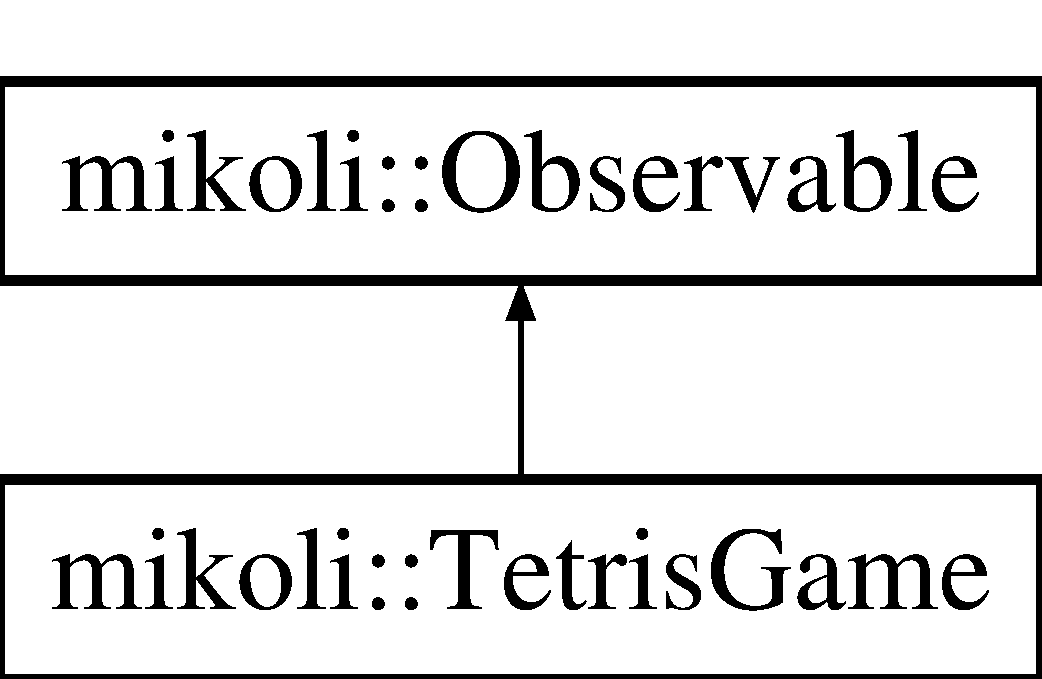
\includegraphics[height=2.000000cm]{classmikoli_1_1_tetris_game}
\end{center}
\end{figure}
\subsection*{Public Member Functions}
\begin{DoxyCompactItemize}
\item 
\mbox{\label{classmikoli_1_1_tetris_game_a45d786fe16165f6c5674e0c2e77d873f}} 
\textbf{ Tetris\+Game} ()
\begin{DoxyCompactList}\small\item\em \doxyref{Tetris\+Game}{p.}{classmikoli_1_1_tetris_game}\textquotesingle{}s constructor without parameter. Build a standard game with level mode \char`\"{}normal\char`\"{} and difficulty \char`\"{}normal\char`\"{}. \end{DoxyCompactList}\item 
\mbox{\label{classmikoli_1_1_tetris_game_a656587e3891ab9e539a2dd48bf135301}} 
\textbf{ Tetris\+Game} (int width, int height)
\begin{DoxyCompactList}\small\item\em \doxyref{Tetris\+Game}{p.}{classmikoli_1_1_tetris_game}\textquotesingle{}s constructor with size parameters. Build a standard game with level mode \char`\"{}normal\char`\"{} and difficulty \char`\"{}normal\char`\"{}. \end{DoxyCompactList}\item 
\mbox{\label{classmikoli_1_1_tetris_game_a79f3e22683d8e7a0f0bf8cc214c6fc11}} 
\textbf{ $\sim$\+Tetris\+Game} ()
\begin{DoxyCompactList}\small\item\em \doxyref{Tetris\+Game}{p.}{classmikoli_1_1_tetris_game} destructor. Deallocate the memory that was previously reserved for the Game. \end{DoxyCompactList}\item 
\textbf{ Figure} \textbf{ get\+Current\+Fig} ()
\begin{DoxyCompactList}\small\item\em get\+Current\+Fig \end{DoxyCompactList}\item 
std\+::vector$<$ \textbf{ Block} $>$ \textbf{ get\+Shadow\+CF} () const
\begin{DoxyCompactList}\small\item\em get\+Shadow\+CF \end{DoxyCompactList}\item 
\textbf{ Figure} \textbf{ get\+Next\+Fig} ()
\begin{DoxyCompactList}\small\item\em get\+Next\+Fig \end{DoxyCompactList}\item 
\textbf{ Board} \textbf{ get\+Board} ()
\begin{DoxyCompactList}\small\item\em get\+Board \end{DoxyCompactList}\item 
bool \textbf{ is\+Game\+Over} ()
\begin{DoxyCompactList}\small\item\em is\+Game\+Over \end{DoxyCompactList}\item 
bool \textbf{ is\+Won} ()
\begin{DoxyCompactList}\small\item\em is\+Won \end{DoxyCompactList}\item 
int \textbf{ get\+Score} ()
\begin{DoxyCompactList}\small\item\em get\+Score \end{DoxyCompactList}\item 
int \textbf{ get\+Level} ()
\begin{DoxyCompactList}\small\item\em get\+Level \end{DoxyCompactList}\item 
int \textbf{ get\+Nb\+Lines} ()
\begin{DoxyCompactList}\small\item\em get\+Nb\+Lines \end{DoxyCompactList}\item 
\textbf{ Mode} \textbf{ get\+Mode} ()
\begin{DoxyCompactList}\small\item\em get\+Mode \end{DoxyCompactList}\item 
bool \textbf{ is\+Begin} ()
\begin{DoxyCompactList}\small\item\em is\+Begin \end{DoxyCompactList}\item 
bool \textbf{ is\+Paused} ()
\begin{DoxyCompactList}\small\item\em is\+Paused \end{DoxyCompactList}\item 
int \textbf{ get\+Speed} ()
\begin{DoxyCompactList}\small\item\em statut\+Speed \end{DoxyCompactList}\item 
bool \textbf{ get\+Is\+Falling} ()
\begin{DoxyCompactList}\small\item\em statut\+Is\+Falling \end{DoxyCompactList}\item 
\mbox{\label{classmikoli_1_1_tetris_game_a4cd2ff57abb9ceee0f42619851b12abd}} 
bool {\bfseries check\+If\+Is\+Blocked} ()
\item 
\textbf{ Timer} $\ast$ \textbf{ get\+Timer} ()
\begin{DoxyCompactList}\small\item\em get\+Timer \end{DoxyCompactList}\item 
\mbox{\label{classmikoli_1_1_tetris_game_a6836c2950a85bbfd715a59475f9a82f4}} 
void \textbf{ is\+Win} ()
\begin{DoxyCompactList}\small\item\em is\+Win Check if the conditions of win are completed. \end{DoxyCompactList}\item 
void \textbf{ move} (Direction direction)
\begin{DoxyCompactList}\small\item\em move \end{DoxyCompactList}\item 
void \textbf{ rotate} (Direction direction)
\begin{DoxyCompactList}\small\item\em rotate \end{DoxyCompactList}\item 
\mbox{\label{classmikoli_1_1_tetris_game_a6f6eb76f89b135a6a58daa3054fd6951}} 
void \textbf{ fall} ()
\begin{DoxyCompactList}\small\item\em fall \end{DoxyCompactList}\item 
\mbox{\label{classmikoli_1_1_tetris_game_a1fe4705ee285f6d8229926fef35c63a8}} 
void \textbf{ fall\+Slow} ()
\begin{DoxyCompactList}\small\item\em fall\+Slow \end{DoxyCompactList}\item 
void \textbf{ end\+Move} (int nb\+Drop)
\begin{DoxyCompactList}\small\item\em end\+Move \end{DoxyCompactList}\item 
\mbox{\label{classmikoli_1_1_tetris_game_a7d3c96ed27130ce1bf8f227c1e764d88}} 
void \textbf{ end\+Game} ()
\begin{DoxyCompactList}\small\item\em end\+Game Stop the \char`\"{}tetris\char`\"{} music and play the \char`\"{}game over\char`\"{} sound, replace all the blocks from the board with grey blocks. \end{DoxyCompactList}\item 
\mbox{\label{classmikoli_1_1_tetris_game_a1d880f26d4e1c364ea502f2298f0ef76}} 
void \textbf{ calculate\+Shadow} ()
\begin{DoxyCompactList}\small\item\em calculate\+Shadow Calcul the positions of the shadow according to the positions of the current figure. \end{DoxyCompactList}\item 
\mbox{\label{classmikoli_1_1_tetris_game_a027e2933909131c71384d311c594c000}} 
void \textbf{ switch\+Pause} ()
\begin{DoxyCompactList}\small\item\em switch\+Pause Switch the game into paused / not paused mode. \end{DoxyCompactList}\item 
void \textbf{ set\+Is\+Begin} (bool \textbf{ is\+Begin})
\begin{DoxyCompactList}\small\item\em set\+Is\+Begin \end{DoxyCompactList}\item 
void \textbf{ set\+Is\+Falling} (bool is\+Falling)
\begin{DoxyCompactList}\small\item\em set\+Is\+Falling \end{DoxyCompactList}\item 
void \textbf{ set\+Auto\+Down} (bool auto\+Down)
\begin{DoxyCompactList}\small\item\em set\+Auto\+Down \end{DoxyCompactList}\item 
\mbox{\label{classmikoli_1_1_tetris_game_a4277c82d6fefaf77c0bc14865c9aa880}} 
void \textbf{ start} ()
\begin{DoxyCompactList}\small\item\em \doxyref{start()}{p.}{classmikoli_1_1_tetris_game_a4277c82d6fefaf77c0bc14865c9aa880} To start the game initialized. Actives the timer and make te \char`\"{}first current figure\char`\"{} moving down. \end{DoxyCompactList}\item 
\mbox{\label{classmikoli_1_1_tetris_game_af0991c69946b7714444644d0c7045512}} 
void \textbf{ start\+With\+Mode} (Gamemode, int)
\begin{DoxyCompactList}\small\item\em start\+With\+Mode Do the same as \doxyref{start()}{p.}{classmikoli_1_1_tetris_game_a4277c82d6fefaf77c0bc14865c9aa880} but change the game mode and the goal. \end{DoxyCompactList}\item 
\mbox{\label{classmikoli_1_1_tetris_game_a56a0258e956f428bfc8ea35ceec1c8ec}} 
void \textbf{ restart} ()
\begin{DoxyCompactList}\small\item\em restart Restart the game\+: reset the score, level, number of lines, board, figure\textquotesingle{}s bag, reset the sounds, reset the attriubutes, ... \end{DoxyCompactList}\end{DoxyCompactItemize}


\subsection{Detailed Description}
The \doxyref{Tetris\+Game}{p.}{classmikoli_1_1_tetris_game} class. 

This class will be used for build a new game.

\+\_\+figures\+Bag The list in which are each figure that will become the next figure and then the current \doxyref{Figure}{p.}{classmikoli_1_1_figure}. \+\_\+current\+Figure The figure that can be rotated or moved during its descent. \+\_\+next\+Figure 

\subsection{Member Function Documentation}
\mbox{\label{classmikoli_1_1_tetris_game_a95b1b5bd20310b52a39f26ea9d0850d1}} 
\index{mikoli\+::\+Tetris\+Game@{mikoli\+::\+Tetris\+Game}!end\+Move@{end\+Move}}
\index{end\+Move@{end\+Move}!mikoli\+::\+Tetris\+Game@{mikoli\+::\+Tetris\+Game}}
\subsubsection{end\+Move()}
{\footnotesize\ttfamily void mikoli\+::\+Tetris\+Game\+::end\+Move (\begin{DoxyParamCaption}\item[{int}]{nb\+Drop }\end{DoxyParamCaption})}



end\+Move 


\begin{DoxyParams}{Parameters}
{\em nb\+Drop} & The number of lines crossed by a fall. Handle the end of a move\+: Add the current figure to the board, check and remove lines if necessary, update the score, change the current figure with the next one, check if the next current figure can be placed in the board, check the conditions of win, ..., call \doxyref{end\+Game()}{p.}{classmikoli_1_1_tetris_game_a7d3c96ed27130ce1bf8f227c1e764d88} is necessary. \\
\hline
\end{DoxyParams}
\mbox{\label{classmikoli_1_1_tetris_game_a45bd5b4cfd5ae69d7fde7122d02f7e8e}} 
\index{mikoli\+::\+Tetris\+Game@{mikoli\+::\+Tetris\+Game}!get\+Board@{get\+Board}}
\index{get\+Board@{get\+Board}!mikoli\+::\+Tetris\+Game@{mikoli\+::\+Tetris\+Game}}
\subsubsection{get\+Board()}
{\footnotesize\ttfamily \textbf{ Board} mikoli\+::\+Tetris\+Game\+::get\+Board (\begin{DoxyParamCaption}{ }\end{DoxyParamCaption})}



get\+Board 

\begin{DoxyReturn}{Returns}
The board. 
\end{DoxyReturn}
\mbox{\label{classmikoli_1_1_tetris_game_ae5f4d4708fd89d37338524c012e56471}} 
\index{mikoli\+::\+Tetris\+Game@{mikoli\+::\+Tetris\+Game}!get\+Current\+Fig@{get\+Current\+Fig}}
\index{get\+Current\+Fig@{get\+Current\+Fig}!mikoli\+::\+Tetris\+Game@{mikoli\+::\+Tetris\+Game}}
\subsubsection{get\+Current\+Fig()}
{\footnotesize\ttfamily \textbf{ Figure} mikoli\+::\+Tetris\+Game\+::get\+Current\+Fig (\begin{DoxyParamCaption}{ }\end{DoxyParamCaption})}



get\+Current\+Fig 

\begin{DoxyReturn}{Returns}
The current figure 
\end{DoxyReturn}
\mbox{\label{classmikoli_1_1_tetris_game_acaf78c2a545806d1bb960056b7e4003c}} 
\index{mikoli\+::\+Tetris\+Game@{mikoli\+::\+Tetris\+Game}!get\+Is\+Falling@{get\+Is\+Falling}}
\index{get\+Is\+Falling@{get\+Is\+Falling}!mikoli\+::\+Tetris\+Game@{mikoli\+::\+Tetris\+Game}}
\subsubsection{get\+Is\+Falling()}
{\footnotesize\ttfamily bool mikoli\+::\+Tetris\+Game\+::get\+Is\+Falling (\begin{DoxyParamCaption}{ }\end{DoxyParamCaption})}



statut\+Is\+Falling 

\begin{DoxyReturn}{Returns}
True if the current figure is falling. 
\end{DoxyReturn}
\mbox{\label{classmikoli_1_1_tetris_game_a327039d28495539cdfccbc5da8ebcb46}} 
\index{mikoli\+::\+Tetris\+Game@{mikoli\+::\+Tetris\+Game}!get\+Level@{get\+Level}}
\index{get\+Level@{get\+Level}!mikoli\+::\+Tetris\+Game@{mikoli\+::\+Tetris\+Game}}
\subsubsection{get\+Level()}
{\footnotesize\ttfamily int mikoli\+::\+Tetris\+Game\+::get\+Level (\begin{DoxyParamCaption}{ }\end{DoxyParamCaption})}



get\+Level 

\begin{DoxyReturn}{Returns}
The current level. 
\end{DoxyReturn}
\mbox{\label{classmikoli_1_1_tetris_game_a3921b5645aeb92a001c9fa6abbb2edad}} 
\index{mikoli\+::\+Tetris\+Game@{mikoli\+::\+Tetris\+Game}!get\+Mode@{get\+Mode}}
\index{get\+Mode@{get\+Mode}!mikoli\+::\+Tetris\+Game@{mikoli\+::\+Tetris\+Game}}
\subsubsection{get\+Mode()}
{\footnotesize\ttfamily \textbf{ Mode} mikoli\+::\+Tetris\+Game\+::get\+Mode (\begin{DoxyParamCaption}{ }\end{DoxyParamCaption})}



get\+Mode 

\begin{DoxyReturn}{Returns}
The mode of the game. 
\end{DoxyReturn}
\mbox{\label{classmikoli_1_1_tetris_game_a3ed7f9da5bdf23792204cb410bb748df}} 
\index{mikoli\+::\+Tetris\+Game@{mikoli\+::\+Tetris\+Game}!get\+Nb\+Lines@{get\+Nb\+Lines}}
\index{get\+Nb\+Lines@{get\+Nb\+Lines}!mikoli\+::\+Tetris\+Game@{mikoli\+::\+Tetris\+Game}}
\subsubsection{get\+Nb\+Lines()}
{\footnotesize\ttfamily int mikoli\+::\+Tetris\+Game\+::get\+Nb\+Lines (\begin{DoxyParamCaption}{ }\end{DoxyParamCaption})}



get\+Nb\+Lines 

\begin{DoxyReturn}{Returns}
The current number of lines made. 
\end{DoxyReturn}
\mbox{\label{classmikoli_1_1_tetris_game_aeda81fb5365aa9900da78d339adf10d1}} 
\index{mikoli\+::\+Tetris\+Game@{mikoli\+::\+Tetris\+Game}!get\+Next\+Fig@{get\+Next\+Fig}}
\index{get\+Next\+Fig@{get\+Next\+Fig}!mikoli\+::\+Tetris\+Game@{mikoli\+::\+Tetris\+Game}}
\subsubsection{get\+Next\+Fig()}
{\footnotesize\ttfamily \textbf{ Figure} mikoli\+::\+Tetris\+Game\+::get\+Next\+Fig (\begin{DoxyParamCaption}{ }\end{DoxyParamCaption})}



get\+Next\+Fig 

\begin{DoxyReturn}{Returns}
The next figure. 
\end{DoxyReturn}
\mbox{\label{classmikoli_1_1_tetris_game_a2ec6092c198e4fc4d94198733969ae5f}} 
\index{mikoli\+::\+Tetris\+Game@{mikoli\+::\+Tetris\+Game}!get\+Score@{get\+Score}}
\index{get\+Score@{get\+Score}!mikoli\+::\+Tetris\+Game@{mikoli\+::\+Tetris\+Game}}
\subsubsection{get\+Score()}
{\footnotesize\ttfamily int mikoli\+::\+Tetris\+Game\+::get\+Score (\begin{DoxyParamCaption}{ }\end{DoxyParamCaption})}



get\+Score 

\begin{DoxyReturn}{Returns}
The current score. 
\end{DoxyReturn}
\mbox{\label{classmikoli_1_1_tetris_game_a1986343731ba85da145114128a098ded}} 
\index{mikoli\+::\+Tetris\+Game@{mikoli\+::\+Tetris\+Game}!get\+Shadow\+CF@{get\+Shadow\+CF}}
\index{get\+Shadow\+CF@{get\+Shadow\+CF}!mikoli\+::\+Tetris\+Game@{mikoli\+::\+Tetris\+Game}}
\subsubsection{get\+Shadow\+C\+F()}
{\footnotesize\ttfamily std\+::vector$<$ \textbf{ Block} $>$ mikoli\+::\+Tetris\+Game\+::get\+Shadow\+CF (\begin{DoxyParamCaption}{ }\end{DoxyParamCaption}) const}



get\+Shadow\+CF 

\begin{DoxyReturn}{Returns}
A vector with the blocks of the shadow. 
\end{DoxyReturn}
\mbox{\label{classmikoli_1_1_tetris_game_a33b6a79e9f92c845f8e993b14e73b0bb}} 
\index{mikoli\+::\+Tetris\+Game@{mikoli\+::\+Tetris\+Game}!get\+Speed@{get\+Speed}}
\index{get\+Speed@{get\+Speed}!mikoli\+::\+Tetris\+Game@{mikoli\+::\+Tetris\+Game}}
\subsubsection{get\+Speed()}
{\footnotesize\ttfamily int mikoli\+::\+Tetris\+Game\+::get\+Speed (\begin{DoxyParamCaption}{ }\end{DoxyParamCaption})}



statut\+Speed 

\begin{DoxyReturn}{Returns}
The actual speed of the game. It\textquotesingle{}s a calcul made according of the level. 
\end{DoxyReturn}
\mbox{\label{classmikoli_1_1_tetris_game_a3b7699d686b8bea0093b4679390131ab}} 
\index{mikoli\+::\+Tetris\+Game@{mikoli\+::\+Tetris\+Game}!get\+Timer@{get\+Timer}}
\index{get\+Timer@{get\+Timer}!mikoli\+::\+Tetris\+Game@{mikoli\+::\+Tetris\+Game}}
\subsubsection{get\+Timer()}
{\footnotesize\ttfamily \textbf{ Timer} $\ast$ mikoli\+::\+Tetris\+Game\+::get\+Timer (\begin{DoxyParamCaption}{ }\end{DoxyParamCaption})}



get\+Timer 

\begin{DoxyReturn}{Returns}
The timer instance with the elapsed time. 
\end{DoxyReturn}
\mbox{\label{classmikoli_1_1_tetris_game_ae7c0b5b7a0ff1534e0e5600f68e90086}} 
\index{mikoli\+::\+Tetris\+Game@{mikoli\+::\+Tetris\+Game}!is\+Begin@{is\+Begin}}
\index{is\+Begin@{is\+Begin}!mikoli\+::\+Tetris\+Game@{mikoli\+::\+Tetris\+Game}}
\subsubsection{is\+Begin()}
{\footnotesize\ttfamily bool mikoli\+::\+Tetris\+Game\+::is\+Begin (\begin{DoxyParamCaption}{ }\end{DoxyParamCaption})}



is\+Begin 

\begin{DoxyReturn}{Returns}
True if the game is began, false otherwise. 
\end{DoxyReturn}
\mbox{\label{classmikoli_1_1_tetris_game_af96f593fdf44d0ef29a595dd46698999}} 
\index{mikoli\+::\+Tetris\+Game@{mikoli\+::\+Tetris\+Game}!is\+Game\+Over@{is\+Game\+Over}}
\index{is\+Game\+Over@{is\+Game\+Over}!mikoli\+::\+Tetris\+Game@{mikoli\+::\+Tetris\+Game}}
\subsubsection{is\+Game\+Over()}
{\footnotesize\ttfamily bool mikoli\+::\+Tetris\+Game\+::is\+Game\+Over (\begin{DoxyParamCaption}{ }\end{DoxyParamCaption})}



is\+Game\+Over 

\begin{DoxyReturn}{Returns}
True is the game is over, false otherwise. 
\end{DoxyReturn}
\mbox{\label{classmikoli_1_1_tetris_game_ac2ff51a7f1de2ba7c2cf84776f41fd28}} 
\index{mikoli\+::\+Tetris\+Game@{mikoli\+::\+Tetris\+Game}!is\+Paused@{is\+Paused}}
\index{is\+Paused@{is\+Paused}!mikoli\+::\+Tetris\+Game@{mikoli\+::\+Tetris\+Game}}
\subsubsection{is\+Paused()}
{\footnotesize\ttfamily bool mikoli\+::\+Tetris\+Game\+::is\+Paused (\begin{DoxyParamCaption}{ }\end{DoxyParamCaption})}



is\+Paused 

\begin{DoxyReturn}{Returns}
True if the game is paused, false otherwise. 
\end{DoxyReturn}
\mbox{\label{classmikoli_1_1_tetris_game_a4835119017717052ba3a0ab9d1ec5297}} 
\index{mikoli\+::\+Tetris\+Game@{mikoli\+::\+Tetris\+Game}!is\+Won@{is\+Won}}
\index{is\+Won@{is\+Won}!mikoli\+::\+Tetris\+Game@{mikoli\+::\+Tetris\+Game}}
\subsubsection{is\+Won()}
{\footnotesize\ttfamily bool mikoli\+::\+Tetris\+Game\+::is\+Won (\begin{DoxyParamCaption}{ }\end{DoxyParamCaption})}



is\+Won 

\begin{DoxyReturn}{Returns}
True if the player reached it\textquotesingle{}s goal, false otherwise. 
\end{DoxyReturn}
\mbox{\label{classmikoli_1_1_tetris_game_ade4c761be1ed35be3bf0c8b26ac5db4f}} 
\index{mikoli\+::\+Tetris\+Game@{mikoli\+::\+Tetris\+Game}!move@{move}}
\index{move@{move}!mikoli\+::\+Tetris\+Game@{mikoli\+::\+Tetris\+Game}}
\subsubsection{move()}
{\footnotesize\ttfamily void mikoli\+::\+Tetris\+Game\+::move (\begin{DoxyParamCaption}\item[{Direction}]{direction }\end{DoxyParamCaption})}



move 


\begin{DoxyParams}{Parameters}
{\em direction} & The direction we want to move. Move the current figure in the direction \char`\"{}direction\char`\"{}. \\
\hline
\end{DoxyParams}
\mbox{\
\section{Time\+Controller Class Reference}
\label{class_time_controller}\index{Time\+Controller@{Time\+Controller}}
Inheritance diagram for Time\+Controller\+:\begin{figure}[H]
\begin{center}
\leavevmode
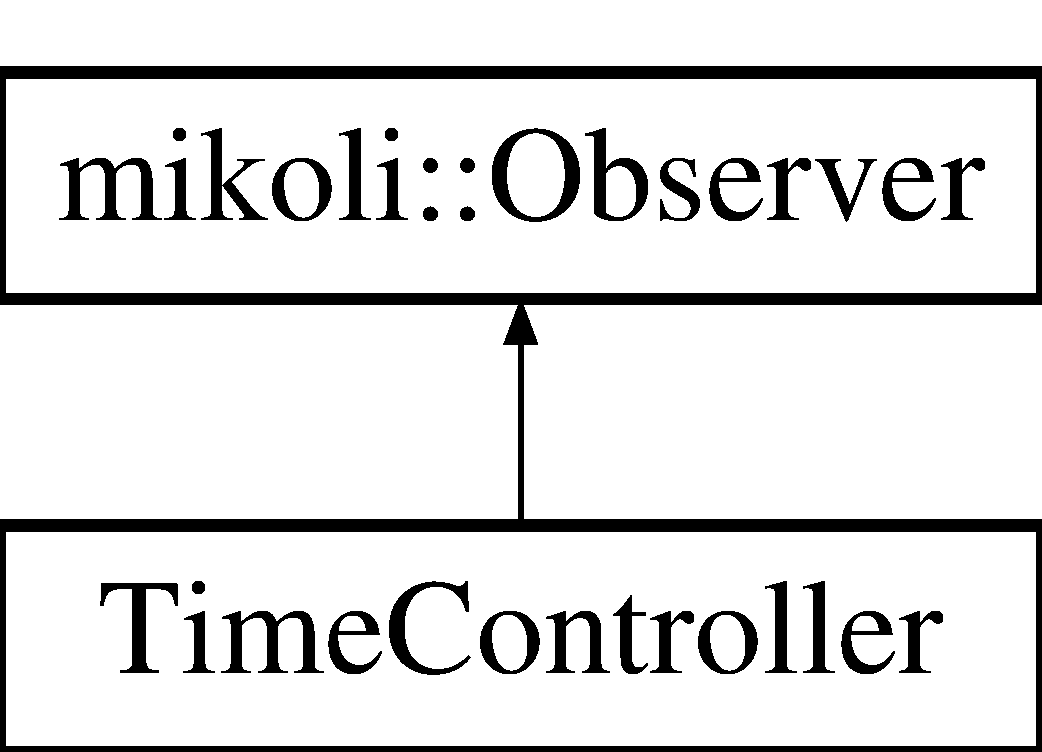
\includegraphics[height=2.000000cm]{class_time_controller}
\end{center}
\end{figure}
\subsection*{Public Member Functions}
\begin{DoxyCompactItemize}
\item 
\mbox{\label{class_time_controller_ab7f47ef57f580761ee0f5dfd72258af7}} 
{\bfseries Time\+Controller} (\textbf{ Widget} \&w)
\item 
\mbox{\label{class_time_controller_a30806fb1b26d4a377bf6ae086efd4ed9}} 
void {\bfseries Update} ()
\end{DoxyCompactItemize}
\subsection*{Friends}
\begin{DoxyCompactItemize}
\item 
\mbox{\label{class_time_controller_a29fa75ce3911bef8c5f4414f6f0242b8}} 
class {\bfseries Widget}
\end{DoxyCompactItemize}
\subsection*{Additional Inherited Members}


The documentation for this class was generated from the following files\+:\begin{DoxyCompactItemize}
\item 
C\+:/\+Users/\+Olivier/\+Desktop/\+Final Tetris cleaned/\+Tetris\+\_\+\+Mikoli/widget.\+h\item 
C\+:/\+Users/\+Olivier/\+Desktop/\+Final Tetris cleaned/\+Tetris\+\_\+\+Mikoli/widget.\+cpp\end{DoxyCompactItemize}

\section{mikoli\+:\+:Timer Class Reference}
\label{classmikoli_1_1_timer}\index{mikoli\+::\+Timer@{mikoli\+::\+Timer}}
Inheritance diagram for mikoli\+:\+:Timer\+:\begin{figure}[H]
\begin{center}
\leavevmode
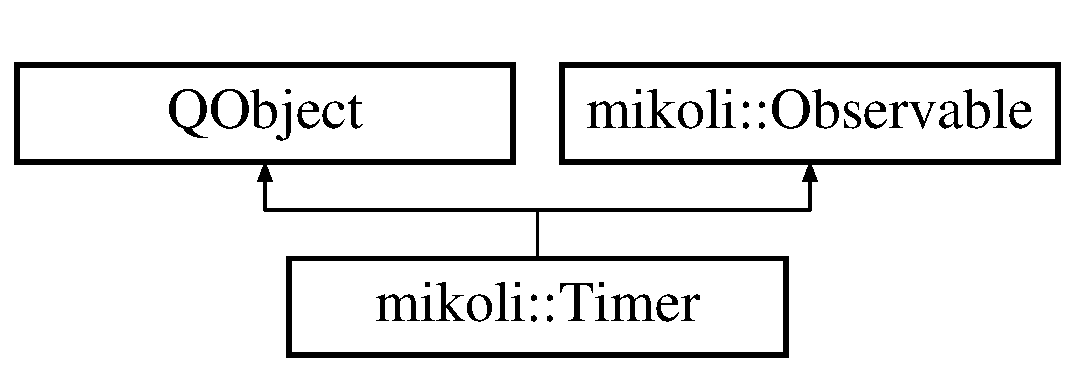
\includegraphics[height=2.000000cm]{classmikoli_1_1_timer}
\end{center}
\end{figure}
\subsection*{Public Slots}
\begin{DoxyCompactItemize}
\item 
\mbox{\label{classmikoli_1_1_timer_a26909e9b17b3de871d821fa4c1ecf656}} 
void \textbf{ My\+Slot} ()
\begin{DoxyCompactList}\small\item\em My\+Slot Inform the view to update the time elapsed view. \end{DoxyCompactList}\end{DoxyCompactItemize}
\subsection*{Public Member Functions}
\begin{DoxyCompactItemize}
\item 
\mbox{\label{classmikoli_1_1_timer_ab3cea51b3631ef452e56ea35448f4864}} 
\textbf{ Timer} ()
\begin{DoxyCompactList}\small\item\em \doxyref{Timer}{p.}{classmikoli_1_1_timer} Constructor by default. \end{DoxyCompactList}\item 
std\+::pair$<$ int, int $>$ \textbf{ statut\+Time\+Game} (void)
\begin{DoxyCompactList}\small\item\em statut\+Time\+Game \end{DoxyCompactList}\item 
int \textbf{ get\+Seconds} ()
\begin{DoxyCompactList}\small\item\em get\+Seconds \end{DoxyCompactList}\item 
int \textbf{ get\+Minutes} ()
\begin{DoxyCompactList}\small\item\em get\+Minutes \end{DoxyCompactList}\item 
int \textbf{ get\+Hours} ()
\begin{DoxyCompactList}\small\item\em get\+Hours \end{DoxyCompactList}\item 
int \textbf{ get\+Total\+Time} ()
\begin{DoxyCompactList}\small\item\em get\+Total\+Time \end{DoxyCompactList}\item 
\mbox{\label{classmikoli_1_1_timer_a0d383f814d81d043295ab804daec8fd7}} 
void \textbf{ play} ()
\begin{DoxyCompactList}\small\item\em play Start the timer. \end{DoxyCompactList}\item 
\mbox{\label{classmikoli_1_1_timer_a7e4452e4c1c9570398983ce97688bb8f}} 
void \textbf{ pause} ()
\begin{DoxyCompactList}\small\item\em pause Pause the timer. \end{DoxyCompactList}\item 
\mbox{\label{classmikoli_1_1_timer_ac45668fc82ca05768f851eae90abd05a}} 
void \textbf{ update\+Duration} ()
\begin{DoxyCompactList}\small\item\em update\+Duration Update the duration attribute \end{DoxyCompactList}\item 
\mbox{\label{classmikoli_1_1_timer_a5e534ac3db890d86a73926b1a9138072}} 
void \textbf{ reset} ()
\begin{DoxyCompactList}\small\item\em reset Reset the timer. \end{DoxyCompactList}\end{DoxyCompactItemize}
\subsection*{Public Attributes}
\begin{DoxyCompactItemize}
\item 
\mbox{\label{classmikoli_1_1_timer_a4e4dd38c46a55ffb0c4385146cabdc6a}} 
Q\+Timer $\ast$ \textbf{ \+\_\+timer}
\begin{DoxyCompactList}\small\item\em \+\_\+timer \doxyref{Timer}{p.}{classmikoli_1_1_timer} that every second, inform the game to update it\textquotesingle{}s view of the time elapsed. \end{DoxyCompactList}\end{DoxyCompactItemize}


\subsection{Member Function Documentation}
\mbox{\label{classmikoli_1_1_timer_acf016e82330d1510af3805238fc11af4}} 
\index{mikoli\+::\+Timer@{mikoli\+::\+Timer}!get\+Hours@{get\+Hours}}
\index{get\+Hours@{get\+Hours}!mikoli\+::\+Timer@{mikoli\+::\+Timer}}
\subsubsection{get\+Hours()}
{\footnotesize\ttfamily int mikoli\+::\+Timer\+::get\+Hours (\begin{DoxyParamCaption}{ }\end{DoxyParamCaption})}



get\+Hours 

\begin{DoxyReturn}{Returns}
The number of hours elapsed. 
\end{DoxyReturn}
\mbox{\label{classmikoli_1_1_timer_a64b031c8a8909b45976490852c9a81ca}} 
\index{mikoli\+::\+Timer@{mikoli\+::\+Timer}!get\+Minutes@{get\+Minutes}}
\index{get\+Minutes@{get\+Minutes}!mikoli\+::\+Timer@{mikoli\+::\+Timer}}
\subsubsection{get\+Minutes()}
{\footnotesize\ttfamily int mikoli\+::\+Timer\+::get\+Minutes (\begin{DoxyParamCaption}{ }\end{DoxyParamCaption})}



get\+Minutes 

\begin{DoxyReturn}{Returns}
The number of minutes elapsed. 
\end{DoxyReturn}
\mbox{\label{classmikoli_1_1_timer_a329669c7864340fb5b2ff971f21d0d75}} 
\index{mikoli\+::\+Timer@{mikoli\+::\+Timer}!get\+Seconds@{get\+Seconds}}
\index{get\+Seconds@{get\+Seconds}!mikoli\+::\+Timer@{mikoli\+::\+Timer}}
\subsubsection{get\+Seconds()}
{\footnotesize\ttfamily int mikoli\+::\+Timer\+::get\+Seconds (\begin{DoxyParamCaption}{ }\end{DoxyParamCaption})}



get\+Seconds 

\begin{DoxyReturn}{Returns}
The number of seconds elapsed. 
\end{DoxyReturn}
\mbox
\section{Ui\+\_\+\+Widget Class Reference}
\label{class_ui___widget}\index{Ui\+\_\+\+Widget@{Ui\+\_\+\+Widget}}
Inheritance diagram for Ui\+\_\+\+Widget\+:\begin{figure}[H]
\begin{center}
\leavevmode
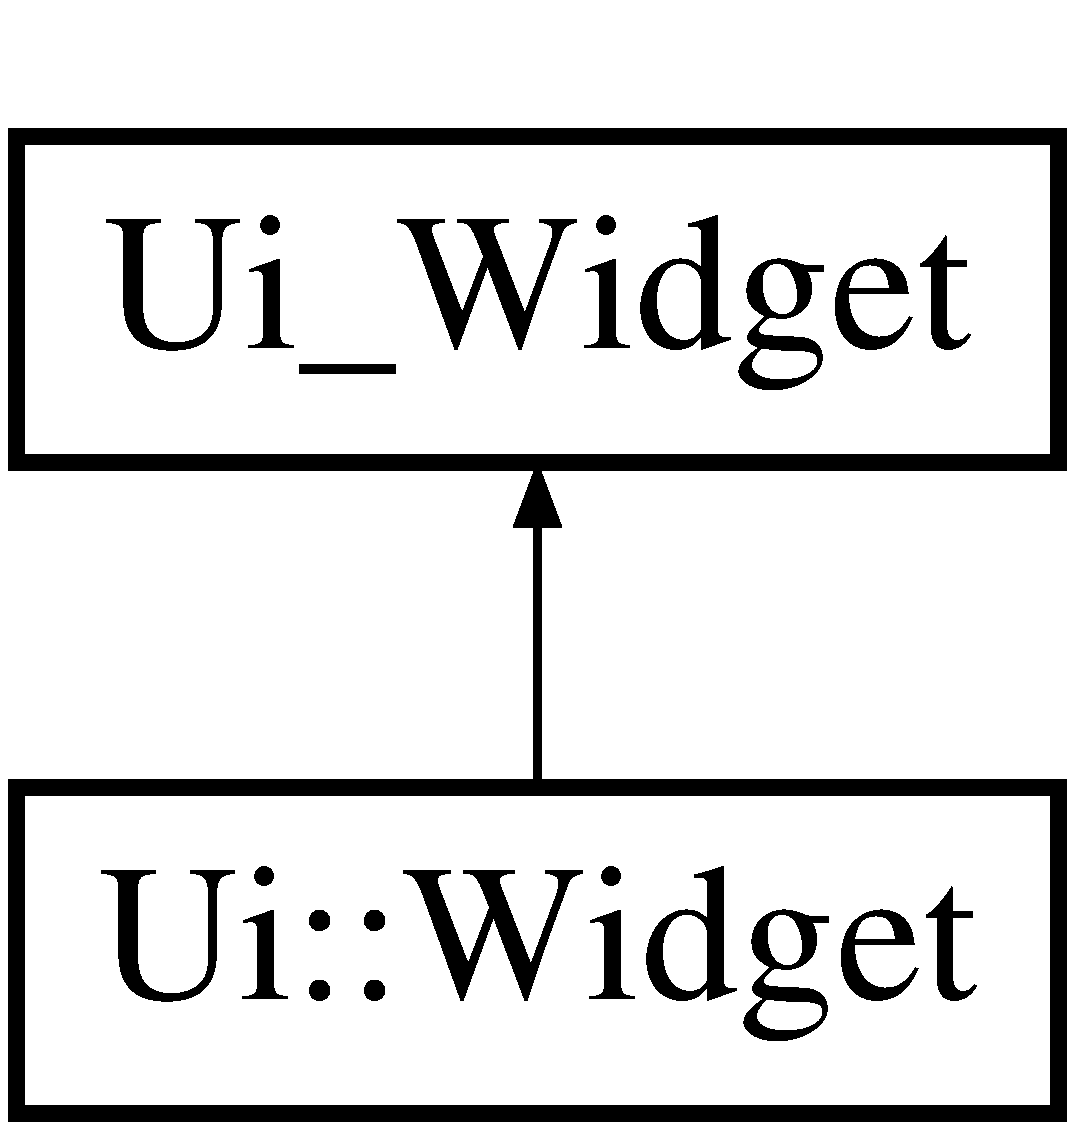
\includegraphics[height=2.000000cm]{class_ui___widget}
\end{center}
\end{figure}
\subsection*{Public Member Functions}
\begin{DoxyCompactItemize}
\item 
\mbox{\label{class_ui___widget_a9039ed8704971418cbe19ef8c9eea266}} 
void {\bfseries setup\+Ui} (Q\+Widget $\ast$\textbf{ Widget})
\item 
\mbox{\label{class_ui___widget_ae1cb85db8d3658df8dcd104361edcecb}} 
void {\bfseries retranslate\+Ui} (Q\+Widget $\ast$\textbf{ Widget})
\end{DoxyCompactItemize}


The documentation for this class was generated from the following file\+:\begin{DoxyCompactItemize}
\item 
C\+:/\+Users/\+Olivier/\+Desktop/\+Final Tetris cleaned/\+Tetris\+\_\+\+Mikoli/ui\+\_\+widget.\+h\end{DoxyCompactItemize}

\section{mikoli\+:\+:View\+Board Class Reference}
\label{classmikoli_1_1_view_board}\index{mikoli\+::\+View\+Board@{mikoli\+::\+View\+Board}}
Inheritance diagram for mikoli\+:\+:View\+Board\+:\begin{figure}[H]
\begin{center}
\leavevmode
\includegraphics[height=2.000000cm]{classmikoli_1_1_view_board}
\end{center}
\end{figure}
\subsection*{Public Member Functions}
\begin{DoxyCompactItemize}
\item 
\mbox{\label{classmikoli_1_1_view_board_af7ed6c813d173fcb07687c0030bf6b06}} 
\textbf{ View\+Board} ()
\begin{DoxyCompactList}\small\item\em The constructor of \doxyref{View\+Board}{p.}{classmikoli_1_1_view_board} without parameter. \end{DoxyCompactList}\item 
\textbf{ View\+Board} (Q\+Widget \&fenetre, \textbf{ Tetris\+Game} \&game)
\begin{DoxyCompactList}\small\item\em The constructor of \doxyref{View\+Board}{p.}{classmikoli_1_1_view_board} with parameters. \end{DoxyCompactList}\item 
\mbox{\label{classmikoli_1_1_view_board_a83b2269ec3fe34b676d9354a3362197c}} 
void \textbf{ set\+Display} ()
\begin{DoxyCompactList}\small\item\em The method called to display the board. \end{DoxyCompactList}\item 
void \textbf{ paint} (\textbf{ Block} bl, int bl\+Size, Q\+Color color, int a, int b, int c, int d, double opacity, bool grad)
\begin{DoxyCompactList}\small\item\em Method to paint blocks with parameters With a relief effect. \end{DoxyCompactList}\item 
\mbox{\label{classmikoli_1_1_view_board_ab1073a80fee01b765d55d48b20d0bba5}} 
void \textbf{ Update} ()
\begin{DoxyCompactList}\small\item\em The method executed when the observable changed. \end{DoxyCompactList}\end{DoxyCompactItemize}
\subsection*{Additional Inherited Members}


\subsection{Constructor \& Destructor Documentation}
\mbox{\label{classmikoli_1_1_view_board_ad3b86ae4358362aaf73eb6a56a4cf44e}} 
\index{mikoli\+::\+View\+Board@{mikoli\+::\+View\+Board}!View\+Board@{View\+Board}}
\index{View\+Board@{View\+Board}!mikoli\+::\+View\+Board@{mikoli\+::\+View\+Board}}
\subsubsection{View\+Board()}
{\footnotesize\ttfamily mikoli\+::\+View\+Board\+::\+View\+Board (\begin{DoxyParamCaption}\item[{Q\+Widget \&}]{fenetre,  }\item[{\textbf{ Tetris\+Game} \&}]{game }\end{DoxyParamCaption})}



The constructor of \doxyref{View\+Board}{p.}{classmikoli_1_1_view_board} with parameters. 


\begin{DoxyParams}{Parameters}
{\em fenetre} & the \doxyref{Widget}{p.}{class_widget} in which the Viewboard has to appear \\
\hline
{\em game} & The \doxyref{Tetris\+Game}{p.}{classmikoli_1_1_tetris_game} (observed) \\
\hline
\end{DoxyParams}


\subsection{Member Function Documentation}
\mbox{\label{classmikoli_1_1_view_board_a352c5ca234d8bb12706fffd10a231dc7}} 
\index{mikoli\+::\+View\+Board@{mikoli\+::\+View\+Board}!paint@{paint}}
\index{paint@{paint}!mikoli\+::\+View\+Board@{mikoli\+::\+View\+Board}}
\subsubsection{paint()}
{\footnotesize\ttfamily void mikoli\+::\+View\+Board\+::paint (\begin{DoxyParamCaption}\item[{\textbf{ Block}}]{bl,  }\item[{int}]{bl\+Size,  }\item[{Q\+Color}]{color,  }\item[{int}]{a,  }\item[{int}]{b,  }\item[{int}]{c,  }\item[{int}]{d,  }\item[{double}]{opacity,  }\item[{bool}]{grad }\end{DoxyParamCaption})}



Method to paint blocks with parameters With a relief effect. 


\begin{DoxyParams}{Parameters}
{\em bl} & the block to paint \\
\hline
{\em bl\+Size} & the block\textquotesingle{}s width \\
\hline
{\em color} & the block\textquotesingle{}s color \\
\hline
{\em a} & value used to print the first level of the block painting (position) \\
\hline
{\em b} & value used to print the first level of the block painting (width) \\
\hline
{\em c} & value used to print the second level of the block painting (position) \\
\hline
{\em d} & value used to print the second level of the block painting (width) \\
\hline
{\em opacity} & the opacity of the block painting \\
\hline
\end{DoxyParams}


The documentation for this class was generated from the following files\+:\begin{DoxyCompactItemize}
\item 
C\+:/\+Users/\+Olivier/\+Desktop/\+Final Tetris cleaned/\+Tetris\+\_\+\+Mikoli/viewboard.\+h\item 
C\+:/\+Users/\+Olivier/\+Desktop/\+Final Tetris cleaned/\+Tetris\+\_\+\+Mikoli/viewboard.\+cpp\end{DoxyCompactItemize}

\section{Ui\+:\+:Widget Class Reference}
\label{class_ui_1_1_widget}\index{Ui\+::\+Widget@{Ui\+::\+Widget}}
Inheritance diagram for Ui\+:\+:Widget\+:\begin{figure}[H]
\begin{center}
\leavevmode
\includegraphics[height=2.000000cm]{class_ui_1_1_widget}
\end{center}
\end{figure}
\subsection*{Additional Inherited Members}


The documentation for this class was generated from the following file\+:\begin{DoxyCompactItemize}
\item 
C\+:/\+Users/\+Olivier/\+Desktop/\+Final Tetris cleaned/\+Tetris\+\_\+\+Mikoli/ui\+\_\+widget.\+h\end{DoxyCompactItemize}

\section{Widget Class Reference}
\label{class_widget}\index{Widget@{Widget}}


\doxyref{Widget}{p.}{class_widget} class used to display the Game.  




{\ttfamily \#include $<$widget.\+h$>$}

Inheritance diagram for Widget\+:\begin{figure}[H]
\begin{center}
\leavevmode
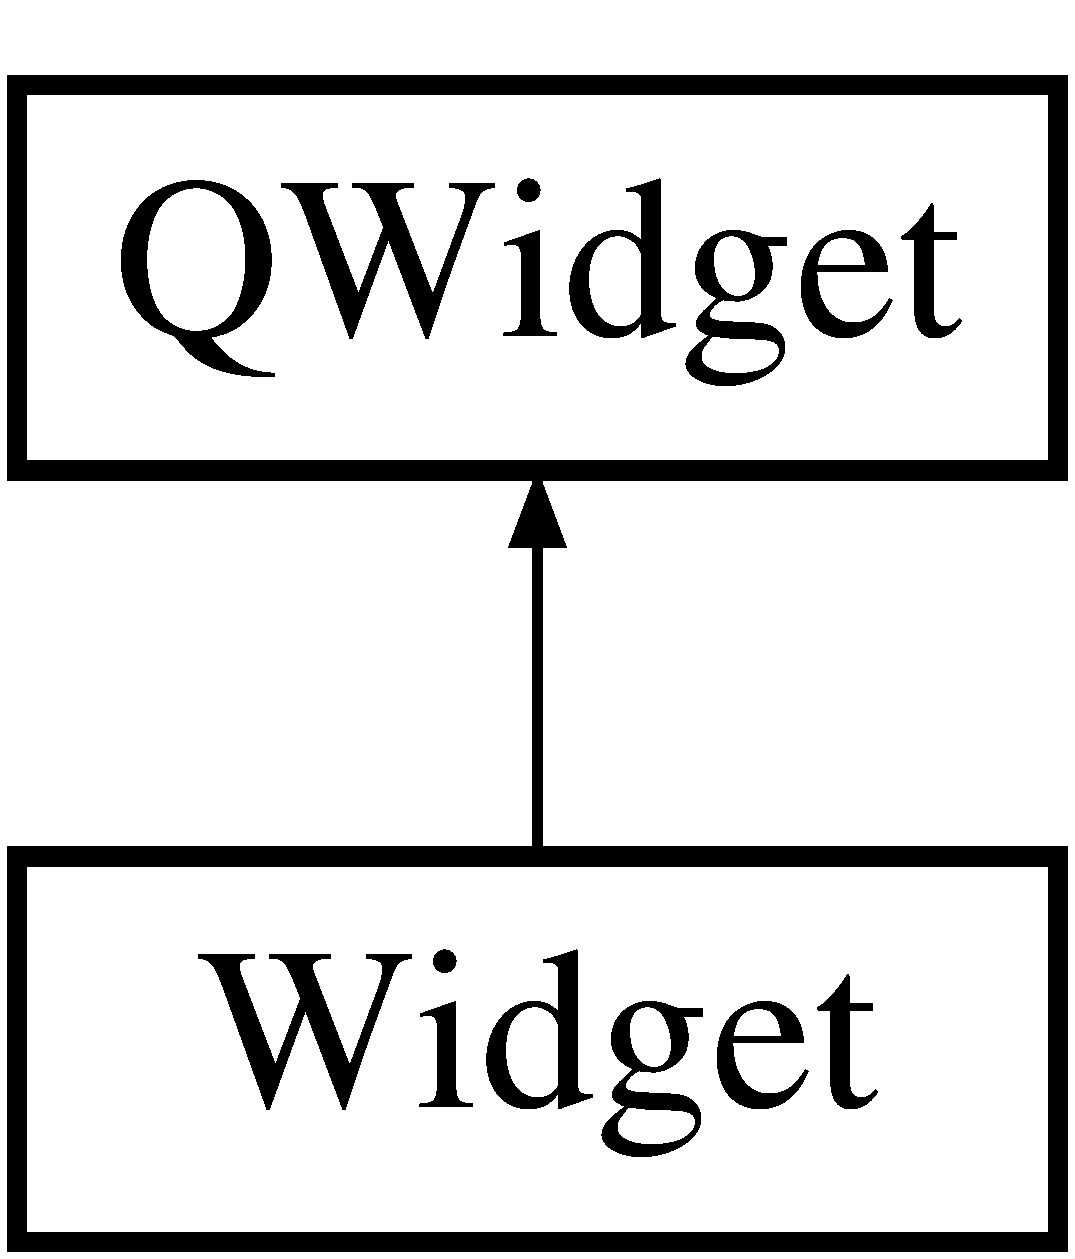
\includegraphics[height=2.000000cm]{class_widget}
\end{center}
\end{figure}
\subsection*{Public Member Functions}
\begin{DoxyCompactItemize}
\item 
\mbox{\label{class_widget_a29531c7f141e461322981b3b579d4590}} 
{\bfseries Widget} (Q\+Widget $\ast$parent=0)
\item 
\mbox{\label{class_widget_aa61c1a3ec57ef894995a052eb7509e1d}} 
\textbf{ Tetris\+Game} \& {\bfseries get\+Game} ()
\end{DoxyCompactItemize}
\subsection*{Public Attributes}
\begin{DoxyCompactItemize}
\item 
\mbox{\label{class_widget_abf94b0570448ffc829aef90f565e2cee}} 
\textbf{ Sound\+Player} $\ast$ {\bfseries \+\_\+start\+Sound}
\item 
\mbox{\label{class_widget_afbbc9a8252e633059d1f1150bde8e47c}} 
\textbf{ Sound\+Player} $\ast$ {\bfseries \+\_\+move\+Sound}
\end{DoxyCompactItemize}
\subsection*{Protected Member Functions}
\begin{DoxyCompactItemize}
\item 
\mbox{\label{class_widget_aa379a46934e5a2246093e5d5b1b1cd72}} 
void {\bfseries timer\+Event} (Q\+Timer\+Event $\ast$event) override
\end{DoxyCompactItemize}
\subsection*{Friends}
\begin{DoxyCompactItemize}
\item 
\mbox{\label{class_widget_af7f0ea7426e91a7ab43bc55cb165bc47}} 
class {\bfseries Time\+Controller}
\end{DoxyCompactItemize}


\subsection{Detailed Description}
\doxyref{Widget}{p.}{class_widget} class used to display the Game. 

The documentation for this class was generated from the following files\+:\begin{DoxyCompactItemize}
\item 
C\+:/\+Users/\+Olivier/\+Desktop/\+Final Tetris cleaned/\+Tetris\+\_\+\+Mikoli/widget.\+h\item 
C\+:/\+Users/\+Olivier/\+Desktop/\+Final Tetris cleaned/\+Tetris\+\_\+\+Mikoli/widget.\+cpp\end{DoxyCompactItemize}

%--- End generated contents ---

% Index
\backmatter
\newpage
\phantomsection
\clearemptydoublepage
\addcontentsline{toc}{chapter}{Index}
\printindex

\end{document}
